% Basic stuff
\documentclass[a4paper,8pt]{extarticle}
\usepackage[utf8]{inputenc}
\usepackage[german]{babel}

% for graphs
\usepackage{pgfplots}
\pgfplotsset{compat=1.5}
\pgfplotsset{width=10cm, height=5cm}

% 3 column landscape layout with fewer margins
\usepackage[landscape, left=0.75cm, top=1cm, right=0.75cm, bottom=1.5cm, footskip=15pt]{geometry}
\usepackage{flowfram}
\ffvadjustfalse
\setlength{\columnsep}{0.75cm}
\Ncolumn{3}

% define nice looking boxes
\usepackage{tcolorbox}

% remove spacing in lists and fancy enumerate
\usepackage{enumitem}
\setlist{noitemsep}

% change section/subsection/... font size
\usepackage{titlesec}
\titleformat*{\section}{\large\bfseries}
\titleformat*{\subsection}{\large\bfseries}


% a base set, that is then customised
\tcbset {
  base/.style={
    boxsep=1pt,left=1pt,right=3pt,top=1pt,bottom=1pt,
    boxrule=0mm,
    leftrule=1mm,
    left=1.75mm,
    arc=0mm, 
    fonttitle=\bfseries, 
    colbacktitle=black!10!white, 
    coltitle=black, 
    toptitle=0.75mm, 
    bottomtitle=0.25mm,
    title={#1}
  }
}

\definecolor{darkorange}{RGB}{255, 127, 0}
\newtcolorbox{mainbox}[1]{
  colframe=darkorange, 
  base={#1}
}

\newtcolorbox{subbox}[1]{
  colframe=black!20!white,
  base={#1}
}

% Bemerkung environment
\newenvironment{bemerkung}{
   \noindent \textbf{Bemerkung:  }}{}

% definition environment
\newenvironment{definition}{
   \noindent \textbf{Definition:  }}{}

   % satz environment
\newenvironment{satz}{
  \noindent \textbf{Satz:  }}{}

% Behauptung environment
\newcounter{behauptung}[section]
\newenvironment{behauptung}{\refstepcounter{behauptung}
   \noindent \textbf{Behauptung~\thesection.\thebehauptung }}{}

% Mathematical typesetting & symbols
\usepackage{amsthm, mathtools, amssymb} 
\usepackage{marvosym, wasysym}

% Tables
\usepackage{tabularx, multirow}
\usepackage{booktabs}
\renewcommand*{\arraystretch}{2}

% Make enumerations more compact
\usepackage{enumitem}
\setitemize{itemsep=0.5pt}
\setenumerate{itemsep=0.75pt}

% To include sketches
\usepackage{graphicx}

% Metadata
\title{\vspace{-1cm}Cheatsheet Analysis 1\vspace{-0.65cm}}
\author{Amos Herz\vspace{-0.5cm}}
\date{FS 2021}

% Math helper stuff
\def\limn{\lim_{n\to \infty}}
\def\sumk{\sum_{k=1}^\infty}
\def\sumn{\sum_{n=0}^\infty}
\def\R{\mathbb{R}}
\def\N{\mathbb{N}}
\def\dx{\text{ d}x}

\begin{document}

\maketitle

\section{Komplexe und Reelle Zahlen}
\subsection{Archimedisches Prinzip}
\begin{mainbox}{Archimedisches Prinzip}
  Sei $x \in \R$ mit $x > 0$ und $y \in \R$. Dann gibt es $n \in \N$ mit $y \leq n \cdot x$.
\end{mainbox}

\subsection{Supremum und Infimum}
\begin{definition}
  $A \subset \R$ heisst von oben [unten] beschränkt falls es $x \in \R$ gibt, sodass $x \geq a$ [$x \leq a$] für alle $a \in A$. $x$ heisst dann obere [untere] Schranke von $A$. Falls $x\in A$ und $x$ obere [untere] SChranke von $A$, ist $x$ das Maximum [Minimum] von $A$.
\end{definition}
\begin{mainbox}{Supremum und Infimum}
  Falls $A \subset \R, A \neq \emptyset$ v.o.b [v.u.b] ist, gibt es eine kleinste obere Schranke [grösste untere Schranke] $x$ von $A$. $x$ heisst dann Supremum [Infimum] von $A$.
\end{mainbox}

\section{Folgen und Reihen}
\subsection{Konvergenz mit $\epsilon$-Def}
\begin{mainbox}{Definition}
  Sei $(a_n)_{n\in \mathbb{N}}$ eine Folge. $(a_n)_{n\in \mathbb{N}}$ konvergiert gegen L \\ $\iff \lim_{n \to \infty} a_n = L $ (i.e. $\exists L \in \R, \forall \epsilon > 0$ die Menge ${n \in \N: a_n \notin ]L - \epsilon, L + \epsilon[}$ endlich ist)\\ $\iff \forall \epsilon > 0 \ \exists N > 1 \ \forall n \ge N : \ | a_n - L | < \epsilon$.
\end{mainbox}
Wir dürfen (o.B.d.A.) annehmen, dass $\epsilon$ durch eine Konstante $C \in \R$ beschränkt ist.
\begin{subbox}{Divergenz}
  Eine Folge $a_n$ ist divergent (notiert $\lim_{n \to \infty} a_n = \infty$) falls: $$\forall K > 0 \exists N = N(K) \in \N \text{, sodass } \forall n \geq N: |a_n| > K$$
\end{subbox}

\subsection{Konvergenz con Folgen}

\begin{bemerkung}
konvergent $\implies$ beschränkt, aber nicht umgekehrt!
\end{bemerkung}\\
\begin{bemerkung}
$(a_n)$ konvergent $\iff (a_n)$ beschränkt \textbf{und} $\lim \inf a_n = \lim \sup a_n$
\end{bemerkung}

\begin{mainbox}{Einschliessungskriterium}
Wenn $\limn a_n = \alpha, \ \limn b_n = \alpha$ und $a_n \le c_n \le b_n, \forall n \ge k$, dann $\limn c_n = \alpha$.
\end{mainbox}

\begin{mainbox}{Weierstrass}
  \begin{itemize}

  \item Sei $a_n$ monoton wachsend und nach oben beschränkt $\Rightarrow a_n$ konvergiert mit Grenzwert $\limn a_n = \sup \{a_n : \ n \ge 1\}$.

  \item $a_n$ monoton fallend und nach unten beschränkt $\Rightarrow$ $a_n$ konvergiert mit Grenzwert $\limn a_n = \inf \{a_n : \ n \ge 1\}$.
  \end{itemize}
\end{mainbox}

\begin{mainbox}{Cauchy-Kriterium}
Eine Folge ($a_n$) heisst \textbf{Cauchy-Folge} falls $\forall \epsilon > 0 \ \exists N \ge 1$ sodass $\forall n,m \ge N_\epsilon$ impliziert, dass
$| a_n - a_m | < \epsilon$.
\end{mainbox}

\begin{bemerkung}
  Für eine Cauchy-Folge $(a_n)$ gilt:
  \begin{itemize}
    \item $(a_n)$ cauchy $\Rightarrow (a_n)$ beschränkt
    \item $(a_n)$ cauchy $\Leftrightarrow (a_n)$ konvergent
  \end{itemize}\leavevmode
\end{bemerkung}

\subsection{Teilfolge}
Eine Teilfolge von $a_n$ ist eine Folge $b_n$ wobei $b_n = a_{l(n)}$ und $l$ eine Funktion mit $l(n) < l(n+1) \quad \forall n \ge 1$ (z.B. $l = 2n$ für jedes gerade Folgenglied). 

\begin{mainbox}{Bolzano-Weierstrass}
  Jede beschränkte Folge besitzt eine konvergente Teilfolge.
\end{mainbox}

\subsection{Limes Superior und Limes Inferior}
\begin{subbox}{Limes superior \& inferior}
  $\limn \inf x_n = \limn \left( \inf_{m \ge n} x_m \right)$ \\
  $\limn \sup x_n = \limn \left( \sup_{m \ge n} x_m \right)$
\end{subbox}

\subsection{Strategie - Konvergenz von Folgen}
\begin{enumerate}
 \item Bei Brüchen: Grösste Potenz von $n$ kürzen. Alle Brüche der Form $\frac{a}{n^a}$ streichen, da diese nach 0 gehen wenn $n \rightarrow 0$.
 \item Bei Wurzeln in Summe im Nenner: Multiplizieren des Nenners und Zählers mit der Differenz der Summe im Nenner. (z.B. $(a+b)$ mit $(a-b)$ multiplizieren)
 \item Bei rekursiven Folgen: Anwendung von Weierstrass zur monotonen Konvergenz
 \item Einschliessungskriterium (Sandwich-Theorem) anwenden.
 \item Mit bekannter Folge vergleichen.
 \item Grenzwert durch einfaches Umformen ermitteln.
 \item Limit per Definition der Konvergenz zeigen.
 \item Anwendung des Cauchy-Kriteriums.
 \item Suchen eines konvergenten Majorant.
 \item Weinen und die Aufgabe überspringen.
\end{enumerate}

\subsection{Strategie - Divergenz von Folgen}
\begin{enumerate}
 \item Suchen einer divergenten Vergleichsfolge.
 \item Bei alternierenden Folgen: Zeige, dass Teilfolgen nicht gleich werden ($\limn a_{p_1(n)} \ne \limn a_{p_2(n)}$), mit z.B. \\ gerade/ungerade als Teilfolgen.
\end{enumerate}

\subsection{Reihe Konvergenz Definition}
\begin{mainbox}{Definition}
  Die Reihe $\sum_{k=1}^\infty a_k$ ist \textbf{konvergent}, falls die Folge $(S_n)_{n \geq 1}$ der Partialsummen konvergiert. In diesem Fall definirien wir: $$\sum_{k=1}^\infty a_k := \lim_{n\to \infty} S_n$$
\end{mainbox}

\subsection{Reihenarithmetik}
\begin{subbox}{Reihenarithmetik}
Wenn $\sumk a_k$ und $\sumk b_k$ konvergent sind, dann gilt:
\begin{itemize}
 \item $\sumk (a_k + b_k)$ konvergent und $\sumk (a_k + b_k) = \left( \sumk a_k \right) + \left( \sumk b_k \right)$
 \item $\sumk \alpha \cdot a_k$ konvergent und $\sumk \alpha \cdot a_k = \alpha \cdot \sumk a_k$
\end{itemize}
\end{subbox}

\subsection{Absolute Konvergenz}
\begin{subbox}{Definition}
$\sumk a_k$ heisst \textbf{absolut konvergent}, falls $\sumk |a_k|$ konvergiert. Eine absolut konvergente Reihe ist auch konvergent, es gilt $$|\sumk a_k| \le \sumk |a_k|$$.
\end{subbox}


\subsection{Konvergenz von Reihen}

\begin{mainbox}{Cauchy-Kriterium für Reihen}
Die Reihe $\sumk a_k$ ist genau dann konvergent, falls $$\forall \epsilon > 0 \ \exists N \ge 1 \ \text{mit} \ | \sum_{k=n}^m a_k | < \epsilon, \ \forall m \ge n > N$$.
\end{mainbox}

\begin{mainbox}{Nullfolgenkriterium}
 Wenn für eine Folge $\limn |a_n| \ne 0$ ist, dann divergiert $\sumn a_n$.
\end{mainbox}
\noindent\textbf{Proof:} 
$a_n$ konvergiert $\Rightarrow s_n = \sum_{i = 1}^n a_i$ konvergiert. Das heisst, es existiert ein Grenzwert $s$, sodass $\lim_{n \to \infty} s_n = s$. Dann gilt:
$$\lim_{n \to \infty} a_n = \lim_{n \to \infty} (s_n - s_{n-1}) = \lim_{n \to \infty} s_n - \lim_{n \to \infty} s_{n-1} = s - s = 0$$


\begin{mainbox}{Vergleichssatz}
Wenn $\sumk a_k$ und $\sumk b_k$ Reihen mit $0 \le a_k \le b_k, \forall k \ge K \ge 1$ sind, so gilt:
$$\sumk b_k \text{ konvergent} \implies \sumk a_k \text{ konvergent}$$ 
$$\sumk a_k \text{ divergent} \implies \sumk b_k \text{ divergent}$$ 
\end{mainbox}

Als Vergleichsreihe (Majorant / Minorant) eignet sich oft eine Reihe der folgenden Kategorien:
\begin{itemize}
  \item \textbf{Geometrische Reihe:} 
  $\sum_{k=0}^\infty q^k$ divergiert für $|q| \ge 1$ und konvergiert zu $\frac{1}{1 - q}$ für $|q| < 1$
  \item \textbf{Zeta-Funktion}
  $\zeta(s) = \sum_{n=1}^\infty \frac{1}{n^s}$ divergiert für $s \le 1$ und konvergiert für $s > 1$.
\end{itemize}

Des weiteren gilt folgendes:
\begin{itemize}
  \item Sei $(S_n) = \sum_{k=0}^\infty q^k$ mit $|q| < 1$, dann ist $(S_n)$ konvergent und $S_n = \frac{1 - q^{n+1}}{1-q}$, \\ $\limn S_n = \frac{1}{1-q}$
  \item $(S_n) = \sum_{k=1}^n \frac{1}{k}$ konvergiert
\end{itemize}

\begin{mainbox}{Leibnizkriterium}
Wenn $a_n \ge 0, \forall n \ge 1$ monoton fallend und $\limn a_n = 0$ ist, dann konvergiert $S = \sum_{k=0}^\infty (-1)^{k} a_k$ und $a_1 - a_2 \le S \le a_1$.
\end{mainbox}

\begin{mainbox}{Quotienten-/Wurzelkriterium}
Sei $(a_n)$ eine Folge mit $a_n \ne 0 \ \forall n \ge 1$. Sei:
\begin{itemize}[nosep]
  \item  $q = \limn \sup \frac{|a_{n+1}|}{|a_n|}$
  \item  $q = \limn \sup \sqrt[n]{|a_n|}$. 
\end{itemize}
Falls gilt:
\begin{itemize}[nosep]
 \item $q < 1 \Rightarrow \sum_{n=1}^\infty a_n$ konvergiert absolut.
 \item $q = 1 \Rightarrow$ keine Aussage.
 \item $q > 1 \Rightarrow \sum_{n=1}^\infty a_n$ divergiert.
\end{itemize}
\end{mainbox}

\subsection{Potenzreihen}
\begin{definition}
  Eine Potenzreihe ist eine Reihe von der Form $\sum_{k = 0}^\infty c_k \cdot z^k$, wobei $(c_k)_{k \geq 0}$ eine Folge ist.
\end{definition}
\begin{mainbox}{Konvergenzradius}
  Der Konvergenzradius $\rho$ einer Potenzreihe entrspricht: $$ \rho \begin{cases}
    + \infty & \text{ falls limsup}_{k \to \infty} \sqrt[k]{|c_k|} = 0\\
    \frac{1}{\text{limsup}_{k \to \infty} \sqrt[k]{|c_k|}} & \text{ falls limsup}_{k \to \infty} \sqrt[k]{|c_k|} > 0
  \end{cases} $$
  DIe Potenzreihe konergiert absolut für alle $|z| < \rho$ und divergiert für alle $|z| > \rho$. Der Fall $|z| = \rho$ musst jeweils noch separat geprüft werden. \\
  EIne Potenzreihe mit positivem Konvergenzradius $\rho$ konvergiert gleichmässig auf $[-\rho, \rho]$, inbesondere ist $f:]-\rho, \rho[\to \R$ stetig.
\end{mainbox}

\subsection{Doppelreihen}

\begin{definition}
  Gegeben eine Doppelfolge $(a_{ij})_{i,j \geq 0}$ so können \\ $\sum_{i=0}^\infty \sum_{j=0}^\infty a_{ij} = A_0 + A_1 + ...$ und $\sum_{j=0}^\infty \sum_{i=0}^\infty a_{ij} = B_0 + B_1 + ...$ beide konvergent sein mit verschiedenen Grenzwerten. Wir nennen $\sum_{i, j \geq 0} a_{ij}$ eine Doppelreihe. Wenn die Reihe bsolut konvergiert, so sind beide Grenzwerte gleich und jere Anordnung knvergiert zum selben Grenzwert.
\end{definition}

\begin{mainbox}{Das Cauchy Produkt}
  Das Cauchy Produkt zweier Reihen $\sum_{i=0}^{\infty} a_i$ und $\sum_{i=0}^{\infty} b_i$ ist die Reihe: 
  $$\sum_{n=0}^{\infty} \sum_{j=0}^\infty (a_{n-j} \cdot b_j) = a_0 b_0 + (a_0 b_1 + a_1 b_0) + ...$$
  Falls beide Reihen \textbf{absolut} konvergieren, so konvergiert auch das Cauchy Produkt und es gilt:
  $$\sum_{n=0}^\infty \left(\sum_{j=0}^n a_{n-j}b_j\right) = \left(\sum_{i=0}^\infty a_i\right) \left(\sum_{j=0}^\infty b_j\right)$$
\end{mainbox}

\subsection{Integral Test}
\begin{mainbox}{Integral Test}
  Sei $f(x)$ eine stetige, positive und monoton fallende Funktion auf $[k, \infty[$ und $f(n) = a_n$:
  $$\int_k^\infty f(x)\dx \text{ konvergiert } \Rightarrow \sum_{n = k}^\infty a_n \text{ konvergiert}$$$$\int_k^\infty f(x)\dx \text{ divergiert } \Rightarrow \sum_{n = k}^\infty a_n \text{ divergiert}$$
\end{mainbox}

\subsubsection{Strategie - Konvergenz von Reihen}
\begin{enumerate}
  \item Ist der Partialsummen nach oben beschränkt? Wenn Ja, konvergiert die Reihe
 \item Ist Reihe ein bekannter Typ? (Teleskopieren, Geometrische/Harmonische Reihe, Zetafunktion, ...)
 \item Ist $\limn a_n = 0$? Wenn nein, divergiert die Reihe (\textit{Nullfolgekriterium})
 \item Quotientenkriterium \& Wurzelkriterium anwenden
 \item Vergleichssatz anwenden, Vergleichsreihen suchen
 \item Leibnizkriterium anwenden
\end{enumerate}

\section{Funktionen und Stetigkeit}
\subsection{Stetigkeit Definitionen}
Sei $f : D \to \R^d, x \to f(x)$ eine Funktion in $D \subseteq \R^d$.
\begin{mainbox}{Definition}
 $f$ ist in $x_0 \in D$ stetig, falls für jede Folge $(a_n)_{n \geq 1}$ mit $\limn a_n = x_0$ folgendes gilt: $$f(\limn a_n) = f(x_0) = \limn f(a_n)$$
 $f$ ist stetig auf D, falls sie in jedem $x_0 \in D$ stetig ist.
\end{mainbox}
\begin{mainbox}{$\epsilon$-Definition}
  \textbf{Punktweise stetig}: $f: D \to \R$ ist stetig in einem Punkt $x_0$ falls: $$\forall \epsilon > 0, \exists \delta > 0, \forall x \in D: |x - x_0| < \delta \Rightarrow |f(x) - f(x_0)| < \epsilon$$
  \textbf{Gleichmässig stetig}: $$\forall \epsilon > 0, \exists \delta > 0, \forall x, x_0 : |x - x_0| < \delta \Rightarrow |f(x) - f(x_0)| < \epsilon$$

 \end{mainbox}
\begin{bemerkung}
  In der punktweisen Stetigkeit ist das $\delta$ von $x_0$ und $\epsilon$ abhängig $(delta(\epsilon, x_0))$, während in der gleichmässigen Stetigkeit das $\delta$ nur von $\epsilon$ abhängen darf $(\delta(\epsilon))$.
\end{bemerkung}
\begin{subbox}{}
 Falls $f$ und $g$ den gleichen Definitions-/Bildbereich haben und in $x_0$ stetig sind, dann sind auch $$f + g, \lambda \cdot f, f \cdot g, \frac{f}{g}, |f|, \max(f,g), \min(f,g)$$ stetig in $x_0$.
\end{subbox}
\begin{bemerkung}
  Polynomiale Funktionen und trigonometrsiche ($\sin$ und $\cos$) Funktionen) sind auf $\R$ stetig.
\end{bemerkung}

\subsection{Zwischenwertsatz}
\begin{mainbox}{Zwischenwertsatz}
 Wenn $I \subseteq \R$ ein Intervall, $f: I \to \R$ und $a, b \in I$ ist, dann gibt es für jedes $c$ zwischen $f(a)$ und $f(b)$ ein $a \le z \le b$ mit $f(z) = c$.
 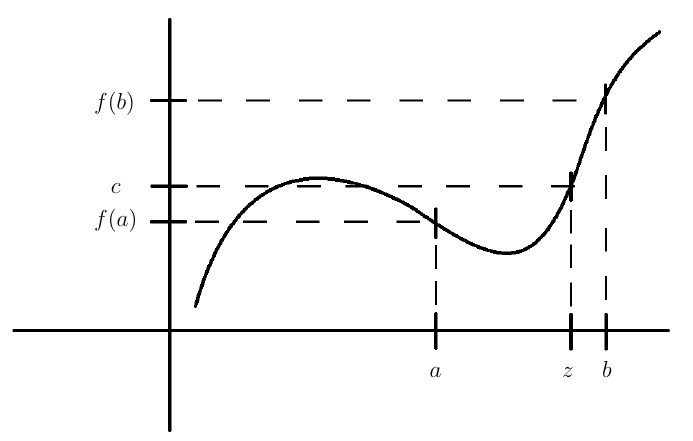
\includegraphics[width=\linewidth]{zwischenwertsatz.png}
 Wird häufig verwendet um zu zeigen, das eine Funktion einen gewissen Wert annimmt.
\end{mainbox}
Daraus folgt, dass ein Polynom mit ungeradem Grad mindestens eine Nullstelle in $\R$ besitzt.

\subsection{Min-Max Satz}
Ein Intervall $I \in \R$ ist kompakt, falls es von der Form $I = [a,b]$ mit $a \le b$ ist.

\begin{mainbox}{Min-Max-Satz}
 Sei $f: I = [a,b] \to \R$ stetig auf einem kompakten Intervall $I$. Dann gibt es $u, v \in I$ mit $$f(u) \le f(x) \le f(v), \forall x \in I$$ Insbesondere ist $f$ \textbf{beschränkt}.
\end{mainbox}

\subsection{Satz über die Umkehrabbildung}
\begin{mainbox}{Satz über die Umkehrabbildung}
 Sei $f: I \to \R$ stetig und streng monoton und sei $J = f(I) \subseteq \R$. Dann ist $f^{-1}: J \to I$ stetig und streng monoton.
\end{mainbox}

\begin{subbox}{Stetigkeit der Verknüpfung}
  Sei $f: D_1 \to D_2, g: D_2 \to \R$ und $x_0 \in D_1$. Falls $f$ in $x_0$ und $g$ in $f(x_0)$ stetig ist, dann ist $g \ocircle f: D_1 \to \R$ in $x_0$ stetig.
 \end{subbox}

\begin{subbox}{Die reelle Exponentialfunktion}
 $\exp: \R \to \ ]0,+\infty[$ ist streng monoton wachsend, stetig und surjektiv. Auch die Umkehrfunktion $\ln: \ ]0,+\infty[ \to \R$ hat diese Eigenschaften.
\end{subbox}

\subsection{Konvergenz von Funktionenfolgen}

\begin{mainbox}{Punktweise Konvergenz}
  Die Funktionenfolge $(f_n)$ konvergiert punktweise gegen eine Funktion $f: D \to \R$ falls für alle $x \in D$ gilt, dass $$\limn f_n(x) = f(x)$$
  \textbf{Alternativ:} $$\forall \epsilon > 0, \forall x \in D, \exists N \geq 1, \forall n \geq N: |f_n(x) - f(x)| < \epsilon$$
\end{mainbox}

\begin{mainbox}{Gleichmässige Konvergenz}
 Die Folge $(f_n)$ konvergiert gleichmässig in $D$ gegen $f$ falls gilt $$\forall \epsilon > 0, \exists N \ge 1, \forall n \ge N, \ \forall x \in D: | f_n(x) - f(x) | \le \epsilon$$
 Die Funktionenfolge $(g_n)$ ist gleichmässig konvergent, falls für alle $x\in D$ der Grenzwert $\limn g_n(x) = g(x)$ existiert und die Folge $(g_n)$ gleichmässig gegen $g$ konvergiert.
\end{mainbox}

\begin{bemerkung}
  In uniform convergence, $N$ does \textbf{not} depend on $x$, we hve to find one which works for all $x$. On the other hand, for pointwise convergence, $N$ can depend on both $\epsilon$ and $x$.
\end{bemerkung}

\begin{bemerkung}
  Wenn eine Funktionenfolge aus stetigen Funktionen besteht und gleichmässig gegen eine Funktion $f$ konvergiert, dann ist $f$ stetig.
\end{bemerkung}

\subsubsection{Strategie: Konvergenz von Funktionenfolgen}
\begin{enumerate}
  \item Punktweiser Limes von $f_n$ auf $D$ finden.
  \item Prüfe auf gleichmässige Konvergenz:
        \begin{enumerate}[label=\roman*]
          \item Indirekte Methode: $f$ unstetig bedeutet keine
          gleichmässige Konvergenz, $f$ stetig, monoton wachsend
          und $D$ kompakt bedeuted gleichmässige Konvergenz.
          \item Direkte Methode: Berechne $sup_{x \in D} |f_n(x) - f(x)|$ (evtl. Ableitung von $|f_n(x) - f(x)|$ gleich Null setzen).
          Danach Limes für $n \to \infty$ von $sup_{x \in D} |f_n(x) - f(x)|$ berechnen, falls dieser Null ist, so konvergiert $f_n$
          gleichmässig.
        \end{enumerate}
  \item Prüfe auf \textbf{nicht} gleichmässige Konvergenz:
        \begin{enumerate}
          \item Assume $\lim_{n \to \infty} f_n(x) = f(x)$.
          \item Choose $x$ and $n$ for which $|f_n(x) - f(x)| \geq \epsilon$ for some $\epsilon$.
        \end{enumerate}
\end{enumerate} 

\subsection{Konvergenz von FunktionenReihen}
\begin{subbox}{}
  Die Reihe $\sumk f_k(x)$ konvergiert gleichmässig, falls die durch $S_n(x) = \sum_{k=0}^n f_k(x)$ definierte Funktionenfolge gleichmässig konvergiert.
\end{subbox}

\begin{subbox}{}
 Sei $f_n$ eine Folge stetiger Funktionen. Ausserdem ist $|f_n(x)| \le c_n \quad \forall x \in D$ und $\sum_{n=0}^\infty c_n$ konvergiert. Dann konvergiert die Reihe $\sum_{n=0}^\infty f_n(x)$ gleichmässig und deren Grenzwert ist eine in $D$ stetige Funktion.
\end{subbox}

\subsection{Potenzreihen}
\begin{subbox}{Potenzreihe}
 Potenzreihen sind Reihen der Form $\sum_{n=0}^\infty a_n x^n$. Eine Potenzreihe mit Entwicklungspunkt $x_0$ wird als $\sum_{n=0}^\infty a_n(x-x_0)^n$ definiert.
\end{subbox}

\begin{mainbox}{Konvergenzradius}
 Der Konvergenzradius einer Potenzreihe um einen Entwicklungspunkt $x_0$ ist die grösste Zahl $r$, so dass die Potenzreihe für alle $x$ mit $|x - x_0| < r$ konvergiert. Falls die Reihe für alle $x$ konvergiert, ist der Konvergenzradius $r$ unendlich. Sonst:
 $$r = \limn \left| \frac{a_n}{a_{n+1}} \right| = \frac{1}{\limn\sup \sqrt[n]{|a_n|}} $$
\end{mainbox}

\subsubsection{Definitionen per Potenzreihen}
\begin{align*}
\exp(x) &= \sumn \frac{x^n}{n!} & r &= \infty \\
\sin(x) &= \sumn (-1)^n \frac{x^{2n + 1}}{(2n + 1)!} & r &= \infty \\
\cos(x) &= \sumn (-1)^n \frac{x^{2n}}{(2n)!} & r &= \infty \\
\ln(x + 1) &= \sumk (-1)^{k+1} \frac{x^k}{k} & r &= 1
\end{align*}

\subsection{Grenzwerte von Funktionen}
\begin{subbox}{Häufungspunkt}
 $x_0 \in \R$ ist ein Häufungspunkt der Menge D falls: $$\forall \delta > 0: (]x_0 - \delta, x_0 + \delta[ \backslash \{x_0\}) \cap D \ne \varnothing$$
\end{subbox}

\begin{mainbox}{Grenzwert - Funktionen}
 Wenn $f: D \to \R, x_0 \in \R$ ein Häufungspunkt von $D$ ist, dann ist $A \in \R$ der Grenzwert von $f(x)$ für $x \to x_0$ ($\lim_{x\to x_0} f(x) = A$), falls $\forall \epsilon > 0 \ \exists \delta > 0$, so dass: $$\forall x \in D \cap (]x_0 - \delta, x_0 + \delta[ \backslash \{x_0\}): |f(x) - A| < \epsilon$$
 \textbf{Alternativ:} $$|f(x) - A| < \epsilon \text{ whenever } 0 < |x - x_0| < \delta$$
\end{mainbox}
\noindent\textbf{Beispiel:}
Prove that $\lim_{x \to 1} (x^2 + 3) = 4$.\\
\textit{Proof:} Begin by letting $\varepsilon > 0$ be given. Find $\delta > 0$ (dependent on $\varepsilon$) so that if $0 < |x - 1| < \delta$, then $|f(x) - 4| < \varepsilon$. Begin with $|f(x) - 4| < \varepsilon$ and solve for $|x - 1|$.\\
$\Rightarrow \ldots \Rightarrow |x-1||x+1| < \varepsilon$.\\
Assume now $\delta \leq 1 \Rightarrow |x - 1| < \delta \leq 1 \Rightarrow -1 < x-1 < 1 \Rightarrow 0 < x < 2$ so that $1 < |x+1| < 3$. \\
Follows $|x-1||x+1| < |x-1| \cdot 3 < \varepsilon \Rightarrow |x-1| < \frac{\epsilon}{3}$. \\
Take now $\delta = \text{min} \{ 1, \frac{\epsilon}{3} \}$. Thus if $0 < |x - 1| < \delta$, it follows that $|f(x) - 10| < \epsilon$.
\begin{subbox}{Limes $\to -\infty / +\infty$}
  $$\lim_{x \to -\infty} [\lim_{x \to +\infty}] f(x) = L$$
  $$\Leftrightarrow |f(x) - L| < \epsilon \ \forall x \in D \text{ with } x < K [x > K]$$
\end{subbox}

\subsection{Linksseitiger und Rechtsseitiger Grenzwert}
Sei $f: D \to \R$ und $x_0 \in D$ ein Häufungspunkt von $D \cap ]x_0, +\infty[$. Falls der Grenzwert der eingeschränkten Funktion $f$ im Bereich $D \cap ]x_0, +\infty[$ für $x \to x_0$ existiert, wird er mit $\lim_{x\to x_0^+}f(x)$ bezeichnet und nennt sich \textbf{rechtsseitiger Grenzwert} von $f$ bei $x_0$. Das Analoge gilt für den \textbf{linksseitigen Grenzwert}. \\
Wir erweitern diese Definition auf $\lim_{x\to x_0^+}f(x) = + \infty$ falls gilt: $$\forall \epsilon > 0, \exists \delta > 0, \forall x \in D \cap ]x_0, x_0 + \delta[: f(x) < \frac{1}{\epsilon}$$
und analog für $\lim_{x\to x_0^+}f(x) = - \infty$ $$\forall \epsilon > 0, \exists \delta > 0, \forall x \in D \cap ]x_0, x_0 + \delta[: f(x) < \frac{1}{-\epsilon}$$
Für den linksseitigen Grenzwert gilt das Analoge. \\
\textbf{Alternativ:} Man sagt $\lim_{x \to x_0^+} f(x) = L$ falls gilt: $$\forall \epsilon \ \exists \delta \ |f(x) - L| < \epsilon \text{ whenever } 0 < x - a < \delta \text{ (oder } a < x  < a + \delta )$$
Man sagt $\lim_{x \to x_0^+} f(x) = L$ falls gilt: $$\forall \epsilon \ \exists \delta \ |f(x) - L| < \epsilon \text{ whenever } -\delta < x - a < 0 \text{ (oder } a - \delta < x  < a )$$

\section{Ableitungen}
\subsection{Differenzierbarkeit}
\begin{mainbox}{Differenzierbar}
 $f$ ist \textbf{in $x_0$ differenzierbar}, falls der Grenzwert $$\lim_{x\to x_0} \frac{f(x) - f(x_0)}{x - x_0} = \lim_{h \to 0} \frac{f(x_0 + h) - f(x_0)}{h}$$ existiert. Wenn dies der Fall ist, wird der Grenzwert mit $f'(x_0)$ oder $\frac{\text{d}f}{\dx}(x0)$ bezeichnet. $f$ ist \textbf{differenzierbar}, falls $f$ für jedes Häufungspunkt $x_0 \in D$ differenzierbar ist.
\end{mainbox}

\begin{bemerkung}
  Die Tangente zu $x_0$ ist definiert durch: $g(x) := f'(x_0) \cdot (x - x_0) + f(x_0)$.
\end{bemerkung}

\begin{subbox}{Differenzierbarkeit nach Weierstrass}
 $f: D \rightarrow R$ ist in $x_0$ differenzierbar ($x_0$ Haufungspunkt von $D$)$\iff$ Es gibt $c \in \R$ und $r: D \to \R$ mit:
 \begin{enumerate}
   \item $f(x) = f(x_0) + c(x - x_0) + r(x) (x - x_0)$ 
   \item $r(x_0) = 0$, $r$ stetig in $x_0$.
 \end{enumerate}
 Falls $f$ differenzierbar ist, dann ist $c = f'(x_0)$ eindeutig bestimmt. \\ \\
 \textbf{Variation}: Eine kunktion $f$ ist genau dann in $x_0$ differenzierbar falls eine Funktion $\phi(x) = f'(x_0) + r(x)$ gibt, so dass $f(x) = f(x_0) + \phi(x) (x-x_0), \ \forall x \in D$ und $\phi$ in $x_0$ stetig ist. In diesem fall gilt $\phi(x_0) = f'(x_0)$.
\end{subbox}
\begin{bemerkung}
  Die Tangentengleichung von $f$ im Punkt $(x_0, f(x_0))$ ist $y = f(x_0) + f'(x_0)(x - x_0)$.
\end{bemerkung}

\begin{mainbox}{Höhere Ableitungen}
 \begin{enumerate}
  \item Für $n \ge 2$ ist $f$ n-mal differenzierbar in $D$ falls $f^{(n-1)}$ in $D$ differenzierbar ist. Dann ist $f^{(n)} = (f^{(n-1)})'$ die n-te Ableitung von $f$.
  \item $f$ ist n-mal stetig differenzierbar in $D$, falls sie n-mal differnzierbar und $f^{(n)}$ in $D$ stetig ist.
  \item $f$ ist in $D$ glatt, falls sie $\forall n \ge 1$ n-mal differenzierbar ist (``unendlich differenzierbar'').
 \end{enumerate}
\end{mainbox}
\begin{bemerkung}
  $\exp(x), \sin(x), \cos(x), \sinh(x), \cosh(x),$ \\ $ \tanh(x), \ln(x), \arcsin(x), \arccos(x), \text{arccot}(x), \arctan(x)$ und alle Polynome sind glatte Funktionen. $\tan(x)$ ist auf $\R \backslash \{\pi/2 + k\pi\}$, $\cot(x)$ auf $\R \backslash \{k\pi\}$ glatt.
\end{bemerkung}
\\
\textbf{Zeigen, dass eine Funktion in $x_{0}$ nicht differenzierbar ist:}
\begin{itemize}
  \item $\lim _{x \rightarrow x_{0}} \frac{f(x)-f\left(x_{0}\right)}{x-x_{0}}=\pm \infty$
  \item $f$ nicht stetig in $x_{0} \Rightarrow f$ nicht differenzierbar in $x_{0}$
  \item $\lim _{x \rightarrow x_{0}^{+}} \frac{f(x)-f\left(x_{0}\right)}{x-x_{0}} \neq \lim _{x \rightarrow x_{0}^{-}} \frac{f(x)-f\left(x_{0}\right)}{x-x_{0}}$
\end{itemize}
\noindent\textbf{Beispiel:} Zeige, dass $\sqrt{x}$ nicht in $x_{0}=0$ differenzierbar ist: \\
$\lim _{h \rightarrow 0} \frac{\sqrt{h}}{h}=\lim _{h \rightarrow 0} \frac{1}{\sqrt{h}}=+\infty$, daher nicht differenzierbar in $x_{0}=0$.

\subsection{Ableitungsregeln}

\begin{subbox}{Linearität der Ableitung}
 $(\alpha \cdot f(x) + g(x))' = \alpha \cdot f'(x) + g'(x)$
\end{subbox}

\begin{mainbox}{Produktregel}
 $(f(x) + g(x))' = f'(x) \cdot g(x) + f(x) \cdot g'(x)$
\end{mainbox}

\begin{mainbox}{Quotientenregel}
 $\left(\frac{f(x)}{g(x)}\right)' = \frac{f'(x) \cdot g(x) - f(x) \cdot g'(x)}{g(x)^2}$
\end{mainbox}

\begin{mainbox}{Kettenregel}
 $(f(g(x)))' = g'(x) \cdot f'(g(x))$
\end{mainbox}

\begin{subbox}{Potenzregel}
 $(c \cdot x^a)' = c \cdot a \cdot x^{a - 1}$
\end{subbox}

\begin{mainbox}{Umkehrfunktion}
  Sei $f(x)$ differenzierbar und invertierbar. 
  $$(f^{-1})'(x) = \frac{1}{f'(f^{-1}(x))}$$
\end{mainbox}

\begin{mainbox}{Rule de L'Hôpital}
Für Grenzwerte, die auf einen unbestimmten Ausdruck der Form $\frac{0}{0}$ oder $\frac{\infty}{\infty}$ führen, gilt:
\begin{equation*}
  \lim_{x\to x_0} \frac{f(x)}{g(x)} = \lim_{x\to x_0} \frac{f'(x)}{g'(x)}
\end{equation*}
\end{mainbox}

\subsection{Hohereableitungsregeln}
Sei $f, g: D \to \R$ $n$-mal differenzierbar.
\begin{subbox}{Linearität der Ableitung}
  $(f + g) ^{(n)} = f^{(n)} + g^{(n)}$
 \end{subbox}
\begin{mainbox}{Produktregel}
  $(f \cdot g)^{(n)} = \sum_{k=0}^n {n \choose k} f^{(k)} \cdot g^{(n-k)}$
 \end{mainbox}
 \begin{bemerkung}
   $\frac{f}{g}$ ist $n$-mal differenzierbar falls $g(x) \neq 0, \forall x \in D$ und $(g \circ f)$ ist $n$-mal differenzierbar.
 \end{bemerkung}

\subsection{Sätze zur Ableitung}
\begin{subbox}{Satz von Rolle}
 Sei $f: [a,b] \to \R$ stetig und in $]a,b[$ differenzierbar. Wenn $f(a) = f(b)$, dann gibt es ein $\xi \in ]a,b[$ mit $f'(\xi) = 0$.
\end{subbox}
\begin{mainbox}{Mittelwertsatz (Lagrange)}
 Sei $f: [a,b] \to \R$ stetig und in $]a,b[$ differenzierbar. Dann gibt es $\xi \in ]a,b[$ mit $f(b) - f(a) = f'(\xi)(b-a) \Leftrightarrow f'(\xi) = \frac{f(b) - f(a)}{b-a}$.
 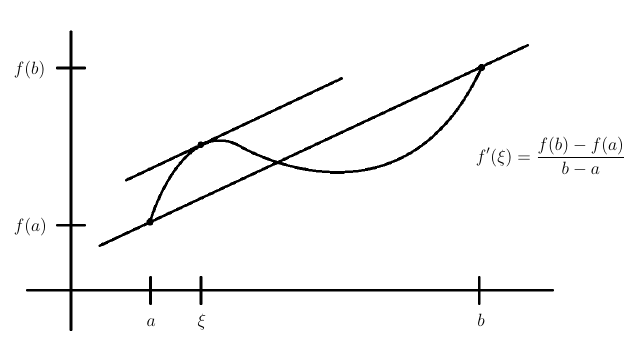
\includegraphics[width=\linewidth]{mittelwertsatz.png}
\end{mainbox}


\subsection{Taylorreihen}
Jede glatte, d.h. beliebig oft differenzierbare, Funktion $f \in C^\infty$ kann als Potenzreihe angenähert werden.

\begin{mainbox}{Taylor-Polynom}
 Das n-te Talyor-Polynom $T_n f(x; a)$ an einer Entwicklungsstelle $a$ ist definiert als:
 $$T_n f(x; a) := \sum_{k=0}^{n} \frac{f^{(k) (a)}}{n!} \cdot (x - a)^k$$ 
 $ = f(a) + f'(a) \cdot (x-a) + \frac{f''(a)}{2} \cdot (x - a)^2 + \ldots$ \\
 mit Rest: $$\frac{f^{n+1}(\xi)}{(n + 1)}(x - a)^{n + 1} \text{ für ein } \xi \in ] a, x [$$ 
\end{mainbox}

\begin{mainbox}{Taylorreihe}
 Die unendliche Reihe
 $$Tf(x;a) := T_\infty = \sumn \frac{f^{(n)}(a)}{n!} \cdot (x-a)^n$$
 wird Taylorreihe von $f$ an Stelle $a$ genannt.
\end{mainbox}
\begin{bemerkung}
  Sei $\sumn c_n x^n$ eine Potenzreihe mit positivem Konvergenzradius $p > 0$. Dann ist $f(x) = \sumn c_l(x - x_0)^n$ auf $]x_0 - p, x_0 + p[$ differenzierbar und $f'(x) = \sumk kc_k(x-x_0)^{k-1}$ für alle $x \in ]x_0 - p, x_0 + p[$.
\end{bemerkung}

\subsection{Kurvendiskussion und Varie}
\subsection{Surjektivität und injektivität}
\begin{mainbox}{Definition}
  Es seien $X$ und $Y$ Mengen, sowie $f: X \rightarrow Y$ eine Abbildung.\\
  \textbf{Surjektivität}: Die Abbildung $f$ heißt surjektiv, wenn es zu jedem  $y \in Y$ (mindestens) ein  $x \in X$ mit $f(x)=y$ gibt. \\
  \textbf{Injektivität}: Die Abbildung $f$ heißt surjektiv, wenn es zu jedem Element $y \in Y$ höchstens ein (also eventuell gar kein) Element $x \in X$ gibt, das darauf zielt, wenn also nie zwei oder mehr verschiedene Elemente der Definitionsmenge auf dasselbe Element der Zielmenge abgebildet werden: $f(x_1)=f(x_2) \Rightarrow x_1=x_2$.
\end{mainbox}

\begin{subbox}{Injektivität zeigen}
  $f$ injektiv $\Leftrightarrow f$ streng monoton $\Leftrightarrow f' > 0$ oder $f' < 0$.
\end{subbox}

\begin{subbox}{Surjektivität zeigen}
  \begin{enumerate}
    \item $\lim_{x\to \infty} f(x) = b $ und $\lim_{x\to -\infty} f(x) = a$ zeigen
    \item Sei nun $y \in]a, b[$ beliebig. Wegen der Grenzwerte von $f$ gilt: $\exists x_1 < x_2 : f(x_1) < y < f(x_2)$. Mit dem Zwischenwertsatz gilt dann: $\exists c \in [x_1, x_2] : f(c) = y$ und somit ist $f$ surjektiv.
  \end{enumerate}
\end{subbox}

\subsubsection{Konvexität und Konkavität}
\begin{mainbox}{Definition}
  $f$ ist [streng] konvex (auf $I$) falls $f$ für alle $x \leq [<] y, x, y \in I$ und $\lambda \in [0, 1]$:
  $$f(\lambda x + (1 - \lambda) y) \ \ \ \ \leq [<] \ \ \ \ \lambda f(x) + (1 - \lambda)f(y)$$
\end{mainbox}
\begin{mainbox}{Bemerkungen}
  \begin{enumerate}
    \item Die Summe zweier konvexer Funktionen ist konvex
    \item $f$ ist genau dann konvex, falls $f$ für $x_0 \leq x \leq x_1$ in $I$ gilt:
          $$\frac{f(x) - f(x_0)}{x - x_0} \leq \frac{f(x_1) - f(x)}{x_1 - x}$$
    \item Die Funktion $f$ ist genau dann [streng] konvex, falls $f'$
          [streng] monoton wachsend ist.  
  \end{enumerate}
\end{mainbox}

\begin{bemerkung}
  Alle Aussagen gelten auch für \textbf{Konkavität}, wir müssen nur das Ungleichzeichen umkehren
\end{bemerkung}

\subsubsection{Begriffe und Korollare}
Es gilt:
\begin{itemize}
  \item $f'(x) = 0 \forall x \Rightarrow f(x)$ konstant
  \item $f'(x) = g'(x) \forall x \Rightarrow \exists c \in \R$ s.t. $f(x) = g(x) + c$
  \item $f'(x) \geq \ (>) \ 0 \forall x \Rightarrow f(x)$ (strikt) monoton wachsend
  \item $f'(x) \leq \ (<) \ 0 \forall x \Rightarrow f(x)$ (strikt) monoton fallend
\end{itemize}

\begin{subbox}{Kritische Punkte}
  Punkte in welchen $f'(x) = 0$ gilt oder $f'(x), f(x)$ nicht existieren, nennen wir kritische Punkte.
\end{subbox}

\begin{bemerkung}
  \begin{itemize}
    \item $n$ gerade und $x_0$ lokale Extremstelle $\Rightarrow f^{(n+1)}(x_0) = 0$
    \item $n$ ungerade und $ f^{(n+1)}(x_0) > 0 \Rightarrow x_0$ eine strikt lokale Minimalstelle
    \item $n$ ungerade und $ f^{(n+1)}(x_0) < 0 \Rightarrow x_0$ eine strikt lokale Maximalstelle
  \end{itemize}
\end{bemerkung}

\subsubsection{Komplette Kurvendiskussion}
\textbf{Symmetrie:}
\begin{itemize}
  \item Achsensymmetrisch/Gerade: \\ $\forall x \in D: f(-x) = f(x)$
  \item Punktsymmetrisch/Ungerade: \\ $\forall x \in D: f(-x) = -f(x)$
\end{itemize}

\textbf{Grenzverhalten:}
\begin{itemize}
  \item Limes für $x \to +\infty$ und $x \to -\infty$ bestimmen
  \item Limes für alle kritische Punkte bestimmen
\end{itemize}

\textbf{Nullstellen:}
\begin{itemize}
  \item Punkte berechnen wo $f(x) = 0$ gilt
  \item Punkte bestimmen wo $f(0) = a$ gilt
\end{itemize}

\textbf{Extremstellen:}
\begin{enumerate}
  \item Berechnung aller kritischen Punkte (u.a.
  (Grenz-) Werte des Intervalls)
  \item Berechnung der ersten Ableitung und der
  Punkte, wo $f'(x_E) = 0$ gilt.
  \item  Berechnung der zweiten Ableitung und von $f''(x_E) = a$:
        \begin{itemize}
          \item $a < 0$: lokales Maximum
          \item $a > 0$: lokales Minimum
          \item $a = 0$: keine Assage moglich
        \end{itemize}
\end{enumerate}

\textbf{Settelpunkte:} Berechnung der Punkte wo gilt:
\begin{itemize}
  \item $f''(x_S) = 0$
  \item $f'''(x_S) \neq 0$
  \item $f'(x_S) \neq 0$
\end{itemize}

\textbf{Wendelpunkte:} Berechnung der Punkte wo gilt:
\begin{itemize}
  \item $f''(x_W) = 0$
  \item $f'''(x_S) \neq 0$
  \item $f'(x_S) = 0$
\end{itemize}

\textbf{Krümmung:} Berechnung der Zweiten Ableitung:
\begin{itemize}
  \item $f''(x) > 0 \rightarrow$ linksgekrümmt (konvex)
  \item $f''(x) < 0 \rightarrow$ rechtsgekrümmt (konkav)
\end{itemize}

\section{Integrale}
\subsection{Riemann-Integral}
\begin{subbox}{Partitionierung}
  Wir teilen das Intervall $I = [a, b]$ in $n$ Teilintervalle auf. Das gibt uns eine Menge von Grenzpunkten $x_0...x_n$. Es gilt also:
  $P := {x_0 = a, x_1, ..., x_{n-1}, x_n = b}$.\\
  Ein Teilintervall $I_i$ ist gegeben durch $I_i =
  [x_{i-1}, x_i]$.
\end{subbox}
\begin{subbox}{Stützstelle}
  Aus jedem Teilintervall $I_i$ wählen wir einen Punkt $\xi_i$. Das gibt uns die Menge der Stützstellen $\xi_1...\xi_n$. \\ $\xi = {\xi_1...\xi_n}$, wobei $\xi_i \in I_i = [x_{i-1}, x_i]$.
\end{subbox}
\begin{mainbox}{Riemann-Summe}
  Gegeben sei eine stetige Funktion $f(x) : [a, b] \rightarrow \R$, sowie eine Partitionierung $P$ in $n$ Teile und Stützstellen $\xi$. Dann ist die Riemannsche Summe definiert durch:
 $$S(f, P, \xi) := \sum_{i=1}^n f(\xi_i) \cdot (x_i - x_{i-1})$$
\end{mainbox}

\begin{subbox}{Ober- und Untersumme}
 Mithilfe der Parition können wir nun die Unertsumme/Obersumme einer Funktion definirien:
 $$s(f, P) = \sum_{i = 1}^n f_i \delta_i, \ \ \ f_i = \inf_{x_{i - 1} \leq x \leq x_i} f(x)$$
 $$S(f, P) = \sum_{i = 1}^n F_i \delta_i, \ \ \ F_i = \sup_{x_{i - 1} \leq x \leq x_i} f(x)$$
 wobei $\delta_i = x_i - x_{i-1}$. \\
 Sei nun $\mathcal{P}(I)$ die Menge alle Partitionen von $I$, definieren wir:
 $$s(f) = \sup_{P \in \mathcal{P}(I)} s(f, P) \ \text{und} \ S(f) = \inf_{P \in \mathcal{P}(I)} S(f, P)$$
\end{subbox}

\begin{mainbox}{Riemann-integrierbar}
 $f:[a,b] \to \R$ ist Riemann-integrierbar, falls $s(f) = S(f)$. In diesem Fall bezeichnen wir den gemeinsamen Wert als: $$s(f) := \int_a^b f(x)\dx = S(f)$$
 \textbf{Alternativ:} $f$ ist genau dann integrierbar wenn gilt: $$\forall \epsilon > 0, \exists P : |s(f, P) - S(f, P)| < \epsilon$$
\end{mainbox}

\begin{bemerkung}
  Sei $\xi_i \in [x_{i-1}, x_i]$ und $m = \max_{1 \leq i \leq n}\{x_i - x_{i-1}\}$. Dann:
  $$\lim_{m \to 0} \sum_{i = 1}^n f(\xi_i) \cdot \delta_i = \int_a^b f(x) \dx$$
  often benutzen wir $\delta_i = \frac{b- a}{n}$ und $\xi_i = a + \left(\frac{b-a}{n}\right)i$ so dass:
  $$\int_a^b f(x) \dx = \lim_{n \to \infty} \sum_{i = 1}^n f(\xi_i) \cdot \delta_i$$
\end{bemerkung}

\begin{bemerkung}
\begin{itemize}
 \item $f$ stetig in $[a,b] \implies f$ integrierbar über $[a,b]$
 \item $f$ monoton in $[a,b] \implies f$ integrierbar über $[a,b]$
\end{itemize}
\end{bemerkung}

\begin{subbox}{}
 Wenn $f,g$ beschränkt und integrierbar sind, dann sind
 $$f+g, \lambda \cdot f, f \cdot g, |f|, \max(f,g), \min(f,g), \frac{f}{g}$$ integrierbar.
\end{subbox}

\noindent \textbf{Beispiel:} Zu zeigen: $f(x) = x^2, x \in [0, 1]$ ist Riemann-inetgrierbar. \\
\textit{Beweis:} Wählen wir $P = [x_0, x_1, \ldots, x_n]$ mit $x_k = \frac{k}{n}, \ k = 0, 1, \ldots, n$ \\
Da $f$ wachsend in $[0, 1]$ für $k = 1, 2, \ldots, n$: 
$$f_i = x_{k-1}^2 = \left(\frac{k-1}{n}\right)^2, \ \ \ F_i = x_k^2 = \left(\frac{k}{n}\right)^2, \ \ \ \delta_i = \frac{1}{n}$$
Jetzt: 
$$s(f, P) = \sum_{k = 1}^n \left(\frac{k-1}{n}\right)^2 \cdot \frac{1}{n} = \ldots = \frac{1}{3} - \frac{3n-1}{6n^2}$$
und $$S(f, P) = \sum_{k = 1}^n \left(\frac{k}{n}\right)^2 \cdot \frac{1}{n} = \ldots = \frac{1}{3} + \frac{3n-1}{6n^2}$$
Da $s(f, P) \leq \frac{1}{3} \leq S(f, P)$ und $S(f, P) - s(f, P) = \frac{1}{n} \to 0 \text{ für } n \to +\infty$, $f$ ist Rieman-integrierbar.

\subsection{Sätze \& Umgleichungen}
\begin{subbox}{Umgleichungen}
\begin{itemize}
 \item $f(x) \le g(x), \forall x \in [a,b] \rightarrow \int_a^b f(x) \dx \le \int_a^b g(x) \dx$
 \item $\left|\int_a^b f(x) \dx\right| \le \int_a^b |f(x)| \dx$
 \item $\left|\int_a^b f(x) g(x) \dx \right| \le \sqrt{\int_a^b f^2(x) \dx} \sqrt{\int_a^b g^2(x) \dx}$
\end{itemize}
\end{subbox}

\begin{mainbox}{Mittelwertsatz}
 Wenn $f: [a,b] \to \R$ stetig ist, dann gibt es $\xi \in [a,b]$ mit $\int_a^b f(x) \dx = f(\xi) (b-a)$.
\end{mainbox}
Daraus folgt auch, dass wenn $f,g: [a,b] \to \R$ wobei $f$ stetig, $g$ beschränkt und integrierbar mit $g(x) \ge 0, \forall x \in [a,b]$ ist, dann gibt es: $$\xi \in [a,b] \ \ \ \ \ \int_a^b f(x)g(x) \dx = f(\xi) \int_a^b g(x) \dx$$

\subsection{Stammfunktionen}
\begin{subbox}{Stammfunktion}
 Eine Funktion $F: [a,b] \to \R$ heisst Stammfunktion von $f$, falls $F$ (stetig) differenzierbar in $[a,b]$ ist und $F' = f$ in $[a,b]$ gilt.
\end{subbox}
\begin{bemerkung}
``$f$ integrierbar'' impliziert \textit{nicht}, dass eine Stammfunktion existiert. Beispiel:
$$
 f(x) = \begin{cases}
        0, & \text{für } x \le 0 \\
        1, & \text{für } x > 0
        \end{cases}
$$
\end{bemerkung}

\begin{mainbox}{Hauptsatz Differential-/Integralrechnung}
 Sei $a<b$ und $f: [a,b] \to \R$ stetig. Die Funktion 
 $$F(x) = \int_a^x f(t) \text{ d}t, \ a \le x \le b$$
 ist in $[a,b]$ stetig differenzierbar und $$F'(x) = f(x) \ \forall x \in [a,b]$$
 Eine äquivalente Darstellung wäre: $$\int_a^b f(x)\dx = F(b) - F(a)$$.
\end{mainbox}

\subsection{Integrationsregeln}
\begin{subbox}{}
  Sei $I \subset R$ ein Intervall und $f : I \rightarrow \R$ stetig. Dann gilt:
  \begin{enumerate}
    \item Seien $a, b, c \in \R$, sodass das abgeschlossene Intervall mit Endpunkten $a + c$, $b + c$ in $I$ enthalten ist:
    $$\int_{a+c}^{b+c} f(x)\dx = \int_a^b f(t + c)\text{d}t$$
    \item Seien $a, b, c \in R$, sodass das abgeschlossene Intervall mit Endpunkten $a \cdot c, b \cdot c$ in $I$ enthalten ist: 
    $$\int_a^b f(ct)\text{d}t = \frac{1}{c}\int_{ac}^{bc} f(x)\dx$$
\end{enumerate}
\end{subbox}
\begin{subbox}{Linearität}
 $$\int u\cdot f(x) + v \cdot g(x) \dx = u \int f(x) \dx + v \int g(x) \dx$$
\end{subbox}
\begin{subbox}{Gebietsadditivität}
 $$\int_a^b f(x) \dx = \int_a^c f(x) \dx + \int_c^b f(x) \dx, \ c \in [a,b]$$
\end{subbox}
\begin{mainbox}{Partielle Integration}
 $$\int f'(x) g(x) \dx = f(x)g(x) - \int f(x) g'(x) \dx$$
\end{mainbox}
\begin{itemize}
 \item Grundsätzlich gilt: Polynome ableiten ($g(x)$), wo das Integral periodisch ist ($\sin, \cos, e^x$,...) integrieren ($f'(x)$)
 \item Teils ist es nötig, mit $1$ zu multiplizieren, um partielle Integration anwenden zu können (z.B. $\int \log(x) \dx$)
 \item Muss eventuell mehrmals angewendet werden
\end{itemize}
\begin{mainbox}{Substitution}
 Um $\int_a^b f(g(x)) \dx$ zu berechnen: Ersetze $g(x)$ durch $u$ und integriere $\int_{g(a)}^{g(b)} f(u) \frac{\text{d}u}{g'(x)}$.
 \\ Auch:
 $$\int_{\phi(a)}^{\phi(b)}f(x)\dx = \int_a^b f(\phi(t))\phi'(t)\text{d}t$$
\end{mainbox}
\begin{itemize}
 \item $g'(x)$ muss sich irgendwie herauskürzen, sonst nutzlos.
 \item Grenzen substituieren nicht vergessen.
 \item Alternativ kann auch das unbestimmte Integral berechnet werden und dann $u$ wieder durch $x$ substituiert werden.
\end{itemize}

\begin{mainbox}{Partialbruchzerlegung}
 Seien $p(x), q(x)$ zwei Polynome. $\int \frac{p(x)}{q(x)}$ wird wie folgend berechnet:
 \begin{enumerate}
  \item Falls $\deg(p) \ge \deg(q)$, führe eine Polynomdivision durch. Dies führt zum Integral $\int a(x) + \frac{r(x)}{q(x)}$.
  \item Berechne die Nullstellen von $q(x)$.
  \item Pro Nullstelle: Einen Partialbruch erstellen.
  \begin{itemize}
   \item Einfach, reell: $x_1 \to \frac{A}{x - x_1}$
   \item $n$-fach, reell: $x_1 \to \frac{A_1}{x - x_1} + \ldots + \frac{A_r}{(x-x_1)^r}$ 
   \item Einfach, komplex: $x^2 + px + q \to \frac{Ax + B} {x^2 + px + q}$
   \item $n$-fach, komplex: $x^2 + px + q \to \frac{A_1x+b_1}{x^2+px+q} + \ldots$
  \end{itemize}
  \item Parameter $A_1, \ldots, A_n$ (bzw. $B_1, \ldots, B_n$) bestimmen. ($x$ jeweils gleich Nullstelle setzen, umformen und lösen).

 \end{enumerate}

\end{mainbox}

\subsection{Integration von konvergenten Reihen}
Sei $f_n : [a, b]\to \R$ eine Folge von beschränkten, integrierbaren Funktionen, die gleichmässig gegen eine Funktion $f: [a, b] \to \R$ konvergiert. Dann ist $f$ beschränkt, integrierbar und es gilt: $$\limn \int_a^b f_n(x)\dx = \int_a^b \limn f_n(x)\dx = \int_a^b f(x)\dx$$
Weiter gilt, wenn $\sum_{n=0}^\infty f_n$ auf $[a, b]$gleichmässig konvergiert $$\sum_{n=0}^\infty \int_a^b f_n(x)\dx = \int_a^b \sum_{n=0}^\infty f_n(x)\dx$$
Sei nun $f(x) = \sum c_kx^k$ eine Potenzreihe mit positivem Konvergenzradius $\rho >0$. Dann ist für jedes $0 \leq r \leq \rho$, $f$ auf $[-r, r]$ integrierbar und es gilt $\forall x \in [-\rho, \rho]$: $$\int_0^x f(t)\text{d}t = \sum_{n=0}^\infty \frac{c_k}{k+1}x^{k+1}$$

\subsection{Euler-McLaurin Formel}
Die Formel hilft Summen wie $1^l + 2^l + 3^l + ... + n^l$ abzuschatzen.
Fur die Formel brauchen wir die Bernoulli Polynome $B_n(x)$,
sowie die Bernoulli Zahlen $B_n(0)$.
Wir brauchen dafur Polynome welche durch die folgenden
Eigenschaften bestimmt sind:

\begin{enumerate}
  \item $P'_k = P_{k-1}, k > 1$
  \item $\int_0^1 P_k(x)\dx = 0, \forall k \geq 1$
\end{enumerate}

Für das $k$-te Bernoulli Polynom gilt: $B_k(x) = k!P_k(x)$. Wir definieren weiter $B_0=1$ und alle anderen Bernoulli Zahlen rekursiv: $B_{k-1} = \sum_{i=0}^{k-1}{k \choose i}B_i = 0$.

Somit erhalten wir für das Bernoulli Polynom folgenden Definition: $$B_k(x) = \sum_{i=0}^{k}{k \choose i}B_ix^{k-i}$$

Bernoulli Polynome und Zahlen:
\begin{center}
\begin{tabular}{c|lc}
  $n$ & $B_n(x)$ & $B_n$ \\
  \hline
  $0$ & $1$ & $1$\\
  $1$ & $x-\frac{1}{2}$ & $\pm \frac{1}{2}$ \\
  $2$ & $x^2-x+\frac{1}{6}$ & $\frac{1}{6}$ \\
  $3$ & $x^3-\frac{3}{2}x^2+\frac{1}{2}x$ & $0$ \\
  $4$ & $x^4-2x^3+x^2-\frac{1}{30}$ & $-\frac{1}{30}$\\
  $5$ & $x^5-\frac{5}{2}x^4+\frac{5}{3}x^3-\frac{1}{6}x$ & $0$\\
  $6$ & $x^6-3x^5+\frac{5}{2}x^4-\frac{1}{2}x^2+\frac{1}{42}$ & $\frac{1}{42}$\\
\end{tabular}
\end{center}
Nun definieren wir noch: $$\tilde{B}_k(x) = \begin{cases}
  B_k(x) & \forall x: 0 \leq x < 1 \\
  B_k(x-n) & \forall x: n \leq x < n + 1
\end{cases}$$

Somit kommen wir aud die Euler-McLaurin Summationsformel:
\begin{mainbox}{Euler-McLaurin Summationsformel}
  Sei $f: [0, n] \to \R$ $k$-mal stetig differenzierbar. Dann gilt: \\
  Für $k = 1$:
  $$\sum_{i = 1}^n f(i) = \int_0^n f(x) \dx + \frac{1}{2}(f(n) - f(0)) + \int_0^n \tilde{B}_1(x)f'(x)\dx$$
  Für $k>1$:
  $$\sum_{i = 1}^n f(i) = \int_0^n f(x) \dx + \frac{1}{2}(f(n) - f(0))+$$
  $$\sum_{j = 2}^k \frac{(-1)^j B_j}{j!}(f^{(j-1)}(n) + f^{(j-1)}(0)) + \tilde{R}_k$$
  wobei
  $$ \tilde{R}_k = \frac{(-1)^{k-1}}{k!} \int_0^n \tilde{B}_k(x)f^{(k)}(x)\dx$$
\end{mainbox}

\begin{subbox}{Example}
  $$1^l + 2^l + 3^l + ... + n^l \text{ wobei } l \geq 1, l \in \N$$
  Angewandt auf $f(x) = x^l$ und $k = l + 1$ folgt für alle $l \geq 1$:
  $$1^l + 2^l + 3^l + ... + n^l = \frac{1}{l + 1} \sum_{j = 0}^l (-1)^j B_j {l + 1 \choose j} n^{l+1-j}$$
\end{subbox}
\subsection{Stirling'sche Formel}
Die Stirling'sche Formel macht eine Aussage über das Verhalten der Fakultät:
$$n! \approx \frac{\sqrt{2 \pi n}\cdot n^n}{e^n} \ \ \text{bzw.} \ \ \limn \frac{n!}{\frac{\sqrt{2 \pi n}\cdot n^n}{e^n}} = 1$$

Wir benützen jetzt die Euler-McLaurin FOrmel um eine präzise Aussage zuerhalten:
\begin{subbox}{}
  $$n! = \frac{\sqrt{2 \pi n}\cdot n^n}{e^n} \cdot \exp\left(\frac{1}{12n} + R_3(n)\right)$$ wobei $$|R_3(n)| \leq \frac{\sqrt{3}}{216} \cdot \frac{1}{n^2} \ \ \forall n \geq 1$$
\end{subbox}

\subsection{Uneigentliche Integral}
\begin{mainbox}{Uneigentliche Integral}
  Sei $f[a, \infty[ \to \R$ beschränkt und integrierbar auf $[a, b]$ für alle $a < b$. Falls: $$ \lim_{b \to \infty} \int_a^b f(x) \dx$$ existiert, wir bezeichnen den Grenzwert mit $$\int_a^\infty f(x)\dx$$ und sagen, dass $f$ auf $[a, \infty[$ integrierbar ist.
\end{mainbox}
Auch hier können wir das Minoranten / Majoranten Kriterium
verwenden. Weiter gilt, dass wenn die Funktion $f: [1, \infty[\to [0, \infty[$monoton fallend ist. Die Reihe genau dann konvergiert, wenn $\int_1^\infty f(x)\dx$ konvergiert.
\begin{mainbox}{}
  $f:]a, b] \to \R$ ist integrierbar, falls: $$\lim_{\epsilon \to 0^+} \int_{a + \epsilon}^bf(x) \dx$$ existiert. In diesem Fall wird der Grenzwert mit $\int_a^b f(x)\dx$ bezeichnet.
\end{mainbox}

\subsection{Gamma Funktion}
DIe Gamma Funktion wir dafür gebraucht um die Funktion $n \mapsto (n-1)!$ zu interpolieren. Für $s > 0$ definieren wir: $$\Gamma(s) := \int_0^\infty e^{-x}x^{s-1}\dx = (s-1)!$$
Die Gamma Funktion konvergiert für alle $s > 0$ und hat folgende weiter Eingeschaften:
\begin{enumerate}
  \item $\Gamma(1) = 1$
  \item $\Gamma(s + 1) = s \Gamma(s)$
  \item $\Gamma$ ist logaritmisch konvex, d.h.: $$\Gamma(\lambda x + (2 - \lambda)y) \leq \Gamma(x)^\lambda \Gamma(y)^{1 - \lambda}$$ für alle $x, y > 0$ und $0 \leq \lambda \leq 1$
\end{enumerate}
Die Gamma Funktion ist die einzige Funktion $]0, \infty[ \to ]0, \infty[$ die $(1), (2)$ und $(3)$ erfüllt. Zudem gilt: $$\Gamma(x) = \limn \frac{n!n^x}{x(x+1)...(x+n)} \ \ \ \forall x > 0$$

\section{Verschiedene Aufgaben}
\begin{enumerate}
  \item Zeige, dass das Chuchy Produkt der beiden ditergenten Reihen $2+2+$ $2^{2}+2^{3}+2^{4}+\cdots$ und $-1+1+1+1+\cdots$ absolut konvergiert. \\
\textit{Beweis:} Wir definieren:
$$
a_{i}= \begin{cases}2, & i=0 \\ 2^{i}, & i=1,2,3,4, \ldots\end{cases}
$$
und
$$
b_{j}= \begin{cases}-1, & j=0 \\ 1, & j=1,2,3,4, \ldots .\end{cases}
$$
und berechnen
$$
\begin{aligned}
\sum_{n=0}^{\infty}\left(\sum_{j=0}^{n} a_{n-j} \cdot b_{j}\right) 
&=a_{0} \cdot b_{0}+\sum_{n=1}^{\infty}\left(\sum_{j=0}^{n} a_{n-j} \cdot b_{j}\right) \\
&=a_{0} \cdot b_{0}+\sum_{n=1}^{\infty}(-2^{n}+2^{n-1}+2^{n-2}+ \\ &\ \ \ \ \ \ +\cdots+2^{1}+2) \\
&=-2+\sum_{n=1}^{\infty}(-2^{n}+2^{n-1}+2^{n-2} \\ &\ \ \ \ \ \ \cdots+2^{1}+2) \\
&=-2+\sum_{n=1}^{\infty}(1+(1+2+2^{2}+\\ &\ \ \ \ \ \ +\cdots+2^{n-1})-2^{n}) \\
&=-2+\sum_{n=1}^{\infty}\left(1+\frac{1-2^{n}}{1-2}-2^{n}\right) \\
&=-2+\sum_{n=1}^{\infty} \underbrace{\left(1-\left(1-2^{n}\right)-2^{n}\right)}_{=0} \\
&=\sum_{n=0}^{\infty} c_{n}, \text { mit } c_{0}=-2 \text { und } c_{n}=0 \ \forall n \geq 1
\end{aligned}
$$
Offensichtlich konvergiert also das Cauchy produkt $\sum_{n=0}^{\infty} c_{n}$
\item Zeige, dast für $a<0$ gilt
$$
\lim _{x \rightarrow 0^{+}} x^{a}=+\infty
$$  \\
\noindent\textit{Beweis:} Wir gehen ähnlich vor wie im Beispiel 3.54. Aus Beispiel 3.53 wissen wir, dass für jedes $n \in \mathbb{N}$ existiert ein $\delta(n)>0$ so, dass
$$
0<x<\delta(n) \Longrightarrow \ln (x)<-n
$$
Jetzt ist aber $a<0$, somit erhalten wir nach multiplizieren mit $a$ die neue Ungleichung
$$
a \ln (x)>-a n
$$
Da exp streng monoton ist, erhalten wir:
$$
x^{n}=\exp \left(\ln \left(x^{n}\right)\right)=\exp (a \ln (x))>\exp (-a n)
$$
und $\mathrm{da}-a n>0$, crhalten wir $\lim _{n \rightarrow \infty} \exp (-a n)=+\infty .$ Nun sei $x_{n}$ cine
positive Nullfolge die gegen 0 strebt. Ohne den Grenzwert von $x_{n}^{4}$ zu verändern, können wit annehmen, dase $0<x_{n}<\delta(n)$. Dann erhalten wir
$$
\lim _{n \rightarrow \infty}\left(x_{a}\right)^{n}>\lim _{n \rightarrow \infty} \exp (-a n)=+\infty
$$
Daraus schliessen wir
$$
\lim _{x \rightarrow 0^{+}} x^{n}=+\infty
$$
\item Sei $f:[0,1] \rightarrow \mathbb{R}$ definiert durch
$$
f(x)= \begin{cases}0, & x=0 \text { oder } x \in \mathbb{R} \mathbb{Q} \\ \frac{1}{q}, & x=\frac{p}{q} \text { , mit } p, q \in \mathbb{N}_{>0} \text{ teilerfremd} \end{cases}
$$
Zeige, dass $f$ integrierbar ist. \\ \\
\textit{Beweis}: Erste Beobachtung: jedes Interval $[x_{i-1}, x_i]$ beinhaltet eine irrationale Zahl, solange $x_{i-1} \neq x_i$. Damit ist für jede Partition $P$ von $[0, 1]$ die Untersumme $s(f, P)$ gleich $0$. \\
Sei $\varepsilon>0$ und $n \in \mathbb{N}$ so dass $\frac{1}{n}<\frac{\varepsilon}{n}$ und $B_{n}$ die Menge aller ``koprimen Brüche'' mit Nenner kleiner gleich $n$ :
$$
B_{\mathrm{a}}=\left\{1, \frac{1}{2}, \frac{1}{3}, \frac{2}{3}, \frac{1}{4}, \frac{3}{4}+\frac{1}{5}, \ldots, \frac{1}{n}, \ldots, \frac{n-1}{n}\right\}
$$
Setze $m=\#B_{n}$, wähle $k>m$ und $P=\left\{x_{0} \ldots, x_k\right\}$ eine Partition mit
$$
\max _{1 \leq i \leq k}\left|x_{i}-x_{i-1}\right|<\frac{e}{4 m},
$$
So eine Partition existiert immer, solange wir $k$ gross genug wählen. Mit der Notation aus der Vorlesung gilt somit
$$P=P_{\frac{\varepsilon}{4m}}$$
Da $B_{n}$ aus $m$ -vielen Elementen besteht. gibt es höchsten $2 m$-viele Intervalle $\left[x_{i-1}, x_{i}\right]$, die $B_{n}$ schneiden. \\
Falls $x \notin B_{a}$. dann ist $x$ entweder irrational (dann folgt $\left.f(x)=0\right), 0$, oder ein Bruch $\frac{p}{q}$ mit $p, q$ teilerfremd und $q>n$ (siehe Definition von $B_{n}$!). Aufjedenfall gilt dann $f(x)<\frac{1}{n}$. \\ 
Wir schätzen nun die Obwerumme $S(f, P)$ von oben ab:

$
\begin{aligned}
  S(f, P) &=\sum_{i=1}^{k}\left(x_{i}-x_{i-1}\right) \cdot \underbrace{\sup _{x \in\left|x_{i}, x_{i-1}\right|} f(x)}_{=f_{i}} \\
  &=\sum_{i \operatorname{mit} \left[x_{i-1}, x_{i}\right] \cap B_{n} \neq 0}\left(x_{i}-x_{i-1}\right) \cdot f_{i} + \\
  &+\sum_{j \operatorname{mit} \left[x_{j-1}, x_{j}\right] \cap B_{n} \neq 0}\left(x_{j}-x_{j-1}\right) \cdot f_{j}
\end{aligned}
$
Die erste Summe läuft höchstens über $2m$ Indizes, da es höchstens soviele Intervalle gibt, die $B_{n}$ schneiden, und es gilt $f_{i} \leq 1$ (weil $\left.f(x) \leq 1\right)$. In der zweiten Summe können wir $f_{i}$ mit $\frac{1}{n}$ abschätzen, da das lntervall $B_{m}$ nicht schneidet und wir $f(y)$ für Element auserthalb von $B_{n}$ mit $\frac{1}{n}$ oben abgesehätzt haben. Auserdem gilt
$$
\begin{aligned}
\sum_{i \operatorname{mit}\left(x_{i-1}, x_{i}\right) \cap B_{n}=0}\left(x_{j}-x_{j-1}\right) &\leq \sum_{j=1}^{k}\left(x_{j}-x_{j-1}\right)\\&=x_{k}-x_{0}=1-0=1
\end{aligned}
$$

Wir werfen alles zusammen und erhalten:
$$
\begin{aligned}
S(f, P) & \leq 2m \cdot \frac{\varepsilon}{4m} \cdot 1+1 \cdot \frac{1}{n} \\
&<\frac{\varepsilon}{2}+\frac{\varepsilon}{2} \\
&=\varepsilon
\end{aligned}
$$
Damit wäre $S(f, P)-s(f, P)<\varepsilon, P=P_{\frac{\varepsilon}{4m}}$
gezeigt, und Satz $5.8$ besagt nun, dass $f$ integrierbar ist.

\item Beweise, dasa falls
$$
\sum_{n=0}^\infty a_nx^n
$$
positive Konvergenzradius besitzt, so ist der Komvergenaradius von
$$
\sum_{0}^{\infty} \frac{a_{n} x^{n}}{n !}
$$
gleich $+\infty$ \\
\textit{Beweis:} Per Definition, ist die Annahme, das $\limsup_{n \to \infty} \sqrt[n]{a_n}$
existiert. Zur Erinnerung
$$\limsup_{n \to \infty} \sqrt[n]{a_n} = \lim_{n \to \infty} \sup_{k \geq n} \sqrt[k]{a_n}$$
Per Definition ist der Konvergenaradius $\rho$ von
$$
\sum_{n=0}^{\infty} \underbrace{\frac{a_{n}}{n !}}_{b_{n}} x^{n}
$$
gleich $+\infty$, genau dann wenn
$$
\limsup_{n \to \infty} \sqrt[n]{\left|b_{n}\right|}=0
$$
Wir zeigen als letzeres:
$$
\begin{aligned}
  \lim _{n \rightarrow \infty} \sup \sqrt[n]{\left|b_{n}\right|} &=\lim _{n \rightarrow \infty} \sup _{k \geq n} \sqrt[k]{\left|b_{k}\right|} \\
  &=\lim _{n \rightarrow \infty} \sup _{k \geq n}\left|a_{k}\right|^{\frac{1}{k}} \cdot k !^{-\frac{1}{k}}
  \end{aligned}
$$
Mit der Stirling'schen Formel gilt
$$
k !^{-1} \approx\left(\frac{\sqrt{2 \pi k} k^{k}}{e^{k}}\right)=\frac{(2 \pi k)^{-\frac{k}{2}} e}{k}=\frac{e}{(\sqrt{2 \pi k})^{k} \cdot k} \rightarrow 0
$$
für $k \rightarrow \infty$. Ausserdem existiert
$$
\lim_{n \to \infty}\underbrace{\sup_{k \geq n} \sqrt[k]{\mid a_{k}\mid}}_{=:c_n}
$$
per Annahme, und somit ist die Folge $c_{n}$ beschränkt. Also existiert eine $C \in \mathbb{R}$ mit $c_{n} \leq C$ für alle $n$, und daher können wir abschätzen:
$$
\begin{aligned}
  \limsup _{n \rightarrow \infty} \sqrt[4]{\left|b_{n}\right|} &=\lim _{n \rightarrow \infty} \sup _{k \geq n}\left|a_{k}\right|^{\frac{1}{k}} \cdot k !^{-\frac{1}{k}} \\
  & \leq \lim _{n \rightarrow \infty} C \cdot k !^{-\frac{1}{k}} \\
  &=C \lim _{n \rightarrow \infty} \sup _{k \geq n} k !^{-\frac{1}{k}} \\
  &=C \cdot \lim _{n \rightarrow \infty} \sup n !^{-\frac{1}{n}} \\
  &=C \cdot \lim _{n \rightarrow \infty} n !^{-\frac{1}{n}} \\
  &=0 .
  \end{aligned}
  $$
Im vorletzten Schritt haben wir verwenden, dass limsup und lim übereinstimmen wenn der Grenzwert existiert.
\end{enumerate}

\section{Trigonometrie} 
\subsection{Hyperbol Funktionen}
\begin{enumerate}
  \item $\sinh(x) := \frac{e^x - e^{-x}}{2} : \R \to \R$
  \item $\cosh(x) := \frac{e^x + e^{-x}}{2} : \R \to [1, \infty[$
  \item $\tanh(x) := \frac{\sinh(x)}{\cosh(x)} = \frac{e^x - e^{-x}}{e^x + e^{-x}} : \R \to [-1, 1[$
\end{enumerate}
\subsection{Regeln}
\subsubsection{Periodizität}
\begin{itemize}
 \item $\sin(\alpha + 2 \pi) = \sin(\alpha) \quad \cos(\alpha + 2 \pi) = \cos(\alpha)$
 \item $\tan(\alpha + \pi) = \tan(\alpha) \quad \cot(\alpha + \pi) = \cot(\alpha)$
\end{itemize}

\subsubsection{Parität}
\begin{itemize}
 \item $\sin(-\alpha) = - \sin(\alpha) \quad \cos(-\alpha) = \cos(\alpha)$
 \item $\tan(-\alpha) = - \tan(\alpha) \quad \cot(-\alpha) = - \cot(\alpha)$
\end{itemize}

\subsubsection{Ergänzung}
\begin{itemize}
 \item $\sin(\pi - \alpha) = \sin(\alpha) \quad \cos(\pi - \alpha) = - \cos(\alpha)$
 \item $\tan(\pi - \alpha) = -\tan(\alpha) \quad \cot(\pi - \alpha) = - \cot(\alpha)$
\end{itemize}


\subsubsection{Komplemente}
\begin{itemize}
 \item $\sin(\pi/2 - \alpha) = \cos(\alpha) \quad \cos(\pi/2 - \alpha) = \sin(\alpha)$
 \item $\tan(\pi/2 - \alpha) = -\tan(\alpha) \quad \cot(\pi/2 - \alpha) = -\cot(\alpha)$
\end{itemize}

\subsubsection{Doppelwinkel}
\begin{itemize}
 \item $\sin(2\alpha) = 2 \sin(\alpha) \cos(\alpha)$
 \item $\cos(2\alpha) = \cos^2(\alpha) - \sin^2(\alpha) = 1 - 2 \sin(\alpha)$
 \item $\tan(2\alpha) = \frac{2\tan(\alpha)}{1 - \tan^2(\alpha)}$
\end{itemize}

\subsubsection{Addition}
\begin{itemize}
 \item $\sin(\alpha + \beta) = \sin(\alpha) \cos(\beta) + \cos(\alpha) \sin(\beta)$
 \item $\cos(\alpha + \beta) = \cos(\alpha) \cos(\beta) - \sin(\alpha) \sin(\beta)$
 \item $\tan(\alpha + \beta) = \frac{\tan(\alpha) + \tan(\beta)}{1 - \tan(\alpha) \tan(\beta)}$
\end{itemize}

\subsubsection{Subtraktion}
\begin{itemize}
 \item $\sin(\alpha - \beta) = \sin(\alpha) \cos(\beta) - \cos(\alpha)\sin(\beta)$
 \item $\cos(\alpha - \beta) = \cos(\alpha) \cos(\beta) + \sin(\alpha)\sin(\beta)$
 \item $\tan(\alpha - \beta) = \frac{\tan(\alpha) - \tan(\beta)}{1+\tan(\alpha) \tan(\beta)}$
\end{itemize}

\subsubsection{Multiplikation}
\begin{itemize}
 \item $\sin(\alpha) \sin(\beta) = -\frac{\cos(\alpha + \beta) - \cos(\alpha - \beta)}{2}$
 \item $\cos(\alpha) \cos(\beta) =  \frac{\cos(\alpha + \beta) + \cos(\alpha - \beta)}{2}$
 \item $\sin(\alpha) \cos(\beta) =  \frac{\sin(\alpha + \beta) + \sin(\alpha - \beta)}{2}$
\end{itemize}

\subsubsection{Potenzen}
\begin{itemize}
 \item $\sin^2(\alpha) = \frac{1}{2}(1-\sin(2\alpha))$
 \item $\cos^2(\alpha) = \frac{1}{2}(1+\cos(2\alpha))$
 \item $\tan^2(\alpha) = \frac{1-\cos(2\alpha)}{1+\cos(2\alpha)}$
\end{itemize}

\subsubsection{Diverse}

\begin{itemize}
 \item $\sin^2(\alpha) + \cos^2(\alpha) = 1$
 \item $\sinh^2(\alpha) - \cosh^2(\alpha) = 1$
 \item $\sin(z) = \frac{e^{iz} - e^{-iz}}{2}$ und $\cos(z) = \frac{e^{iz} + e^{-iz}}{2}$
\end{itemize}


\begin{mainbox}{Wichtige Werte}
\begin{center} 
 \begin{tabular}{c|cccccc}
  deg & 0$^{\circ}$  & 30$^{\circ}$  & 45$^{\circ}$  & 60$^{\circ}$  & 90$^{\circ}$  & 180$^{\circ}$  \\
  \midrule
  rad & 0 & $\frac{\pi}{6}$ & $\frac{\pi}{4}$ & $\frac{\pi}{3}$ & $\frac{\pi}{2}$ & $\pi$ \\
  cos & 1 & $\frac{\sqrt{3}}{2}$ & $\frac{\sqrt{2}}{2}$ & $\frac{1}{2}$ & 0 & -1 \\
  sin & 0 & $\frac{1}{2}$ & $\frac{\sqrt{2}}{2}$ & $\frac{\sqrt{3}}{2}$ & 1 & 0 \\
  tan & 0 & $\frac{1}{\sqrt{3}}$ & 1 & $\sqrt{3}$ & $+\infty$ & 0 \\
 \end{tabular}
\end{center}
\end{mainbox}

\section{Nütziche Sätze}

\begin{subbox}{Bogenlänge}
  $$\mathcal{L} = \int_a^b \sqrt{1 + (f'(x))^2}$$ 
\end{subbox}

\begin{subbox}{Bernoulli Ungleichung}
  $$(1 + x)^n \geq 1 + n \cdot x \ \ \ \forall n \in \mathbb{N}, x > -1$$
\end{subbox}

\begin{subbox}{Young'sche Ungleichung}
  $$\forall \epsilon > 0, \forall x, y \in \R: 2|xy| \leq \epsilon x^2 + \frac{1}{\epsilon} y^2$$
\end{subbox}

\begin{subbox}{Binomialsatz}
  $$(x + y)^n = \sum_{k = 0}^n {n \choose k} x^{n-k}y^k$$
\end{subbox}

\subsection{Komplexe Zahlen}
  $$z = a + b \cdot \,\mathrm i$$
  $$z = r(\cos \omega + \,\mathrm i \sin \omega) = r \text{ cis } \omega = r\cdot e^{\,\mathrm i \omega}$$
  \textbf{Exponent:} $z^n = r^ne^{\,\mathrm i n \omega}$ \\
  For the following let $z_1 = a + \,\mathrm i\cdot b$ and $z_2 = c + \,\mathrm i \cdot d$. 
  \begin{subbox}{Addition/Subtraktion}
    $$z_1+z_2=(a+c)+(b+d)\,\mathrm i \text{   ,   } z_1-z_2=(a-c)+(b-d)\,\mathrm i$$
  \end{subbox}

  \begin{subbox}{Multiplikation}
    $$z_1\cdot z_2=(ac+bd\,\mathrm i^2)+(ad+bc)\,\mathrm i=(ac-bd)+(ad+bc)\,\mathrm i$$
  \end{subbox}

  \begin{subbox}{Division}
    $$\frac{z_1}{z_2} = \frac{(a+b\,\mathrm i)(c-d\,\mathrm i)}{(c+d\,\mathrm i)(c-d\,\mathrm i)} = \frac{ac+bd}{c^2+d^2}+\frac{bc-ad}{c^2+d^2}\mathrm i$$
  \end{subbox}
\subsection{Exponential-Funktion und Logarithmus}
\begin{itemize}
  \item $e \approx 2.72, \ln (1)=0, \ln (e)=1$
  \item  $\exp (x)>0, \forall x \in \mathbb{R}$ und $\exp (x)>1, \forall x>0$
  \item $1+x \leq e^{x}$
  \item $(1+x)^{n} \geq 1+n x$ (Bernoullische Ungleichung)
  \item $|a+b| \leq|a|+|b|$ (Dreiecksungleichung)
  \item $\log (x) \leq \sqrt{x}, \forall x>0$
  \item $\ln (a \cdot b)=\ln (a)+\ln (b)$ und $\ln \left(\frac{a}{b}\right)=\ln (a)-\ln (b)$
  \item $\ln \left(a^{b}\right)=b \cdot \ln (a)$ und $\log _{a}(x)=\frac{\ln (x)}{\ln (a)}$
  \item $e^{\ln (x)}=x$ und $\ln \left(e^{x}\right)=x$
  \item $x^{a}=e^{a \ln (x)}$
\end{itemize}

\subsection{Bekannte Taylorreihen}
\begin{align*}
  e^x = \lim_{n \to \infty} \left(1 + \frac{x}{n} \right)^n & = 1 + x + \frac{x^2}{2!} + \frac{x^3}{3!} + \frac{x^4}{4!} + \mathcal{O}(x^5) \\
  \sin(x) & = x - \frac{x^3}{3!} + \frac{x^5}{5!} - \frac{x^7}{7!} + \mathcal{O}(x^9) \\ 
  \sinh(x) & = x + \frac{x^3}{3!} + \frac{x^5}{5!} + \frac{x^7}{7!} + \mathcal{O}(x^9) \\ 
  \cos(x) & = 1 - \frac{x^2}{2!} + \frac{x^4}{4!} - \frac{x^6}{6!} + \mathcal{O}(x^8) \\  
  \cosh(x) & = 1 + \frac{x^2}{2!} + \frac{x^4}{4!} + \frac{x^6}{6!} + \mathcal{O}(x^8) \\  
  \tan(x) & = x + \frac{x^3}{3} + \frac{2x^5}{15} + \mathcal{O}(x^6) \\ 
  \tanh(x) & = x - \frac{x^3}{3} + \frac{2x^5}{15} + \mathcal{O}(x^6) \\ 
  \ln(1 + x) & = x - \frac{x^2}{2} + \frac{x^3}{3} - \frac{x^4}{4} \mathcal{O}(x^5) \\
  (1 + x)^\alpha & = 1 + \alpha x - \frac{\alpha (\alpha - 1)}{2}x^2 + \mathcal{O}(x^3) \\ 
  \sqrt{1 + x} & = 1 + \frac{x}{2} - \frac{x^2}{8} + \frac{x^3}{16} - \mathcal{O}(x^4) \\
\end{align*}

\subsection{Wichtige Reihen}
\begin{align*}
 \sum_{i=1}^n i &= \frac{n(n+1)}{2} \\
 \sum_{i=1}^n i^2 &= \frac{n(n+1)(2n+1)}{6} \\
 \sum_{i=1}^n i^3 &= \frac{n^2(n+1)^2}{4} \\
 \sum_{i=1}^\infty \frac{1}{i^2} &= \frac{\pi^2}{6} \\
 \sum_{n=1}^\infty \frac{1}{n(n+1)} &= 1
\end{align*}


\section{Tabellen}
\def\limxpi{\lim_{x\to +\infty}}
\def\limxmi{\lim_{x\to -\infty}}
\def\limxi{\lim_{x\to \pm \infty}}
\subsection{Typische Grenzwerte}
\begin{center}
  \begin{tabular}[]{|l|l|}
    \hline
    $\limxpi \frac{1}{x} = 0$ & $\limxpi 1 + \frac{1}{x} = 1$ \\
    \hline
    $\limxmi e^x = +\infty$ & $\limxmi e^x = 0$ \\
    \hline
    $\limxmi e^{-x} = 0$ & $\limxmi e^{-x} = +\infty$ \\
    \hline
    $\limxpi \frac{e^x}{x^m} = +\infty$ & $\limxmi x e^x = 0$ \\
    \hline
    $\limxpi \ln(x) = +\infty$ & $\lim_{x \to 0} \ln(x) = -\infty$ \\
    \hline
    $\limxpi (1 + x)^{\frac{1}{x}} = 1$ & $\lim_{x \to 0} (1 + x)^{\frac{1}{x}} = e$ \\
    \hline
    $\limxpi (1 + \frac{1}{x})^b = 1$ &  $\lim_{x \to 0} (1 + \frac{1}{x})^b = +\infty$\\
    \hline
    $\limxpi x^aq^x = 0, \forall 0 \leq q < 1$ & $\limxpi n^{\frac{1}{n}} = 1$\\
    \hline
    $\limxi (1 + \frac{1}{x})^x = e$ & $\limxi (1 - \frac{1}{x})^x = \frac{1}{e}$ \\
    \hline
    $\limxi (1 + \frac{k}{x})^{mx} = e^{km}$ & $\lim_{x \to 0} \frac{\sin(x)}{x} = 1$ \\
    \hline
    $\lim_{x \to 0} \frac{1}{\cos(x)} = 1$ & $\lim_{x \to 0} \frac{\cos(x) - 1}{x} = 0$ \\
    \hline
    $\lim_{x \to 0} x\log(x) = 0$ & $\lim_{x \to 0} \frac{\log(1) - x}{x} = 1$ \\
    \hline
    $\lim_{x \to 0} \frac{1 - \cos(x)}{x^2} = \frac{1}{2}$ & $\lim_{x \to 0} \frac{e^x - 1}{x} = 1$ \\
    \hline
    $\lim_{x \to 0} \frac{x}{\arctan(x)} = 1$ & $\limxpi \arctan(x) = \frac{\pi}{2}$ \\
    \hline
    $\limxpi \left( \frac{x}{x+k}  \right) ^x = e^{-k}$ & $\lim_{x \to 0} \frac{e^x - 1}{x} = 1$ \\
    \hline
    $\lim_{x \to 0} \frac{a^x - 1}{x} = \ln(a)  \forall a > 0$ & $\lim_{x \to 0} \frac{e^{ax}-1}{x} = a$ \\
    \hline
    $\limxpi \frac{\ln(x)}{x} = 0$ & $\limxpi \frac{\log(x)}{x^a} = 0$ \\
    \hline
    $\limxpi \sqrt[x]{x} = 1$ & $\limxpi \frac{2x}{2^x} = 0$ \\
    \hline
  \end{tabular}
\end{center}
\begin{bemerkung}
  $\lim _{n \rightarrow \infty} \sqrt[n]{x}=1$ für $\forall x>0$
\end{bemerkung}

\subsection{Ableitungen und Stammfunktionen}

\renewcommand\arraystretch{2}

\begin{center}
        \begin{tabular}{|c|c|}
          \hline
                $F(x)$ & $F'(x) = f(x)$ \\
                \hline \hline
                
                $ c $ & $ 0 $ \\
                \hline
	        $ x^a $ & $ a \cdot x^{a - 1} $ \\
          \hline
                $ \frac{1}{a+1} x^{a+1} $ & $ x^a $ \\
                \hline
                $ \frac{1}{a\cdot(n+1)} (ax+b)^{n+1} $ & $ (ax+b)^n $ \\
                \hline
	        $ \frac{x^{\alpha+1}}{\alpha + 1} $ & $ x^\alpha, \alpha \neq -1 $ \\
          \hline
                $ \sqrt x $ & $ \frac{1}{2 \sqrt x} $ \\
                \hline
                $ \sqrt[n] x $ & $ \frac{1}{n} {x}^{ \frac{1}{n} -1 } $ \\
                \hline
                $ \frac{2}{3} x^{ \frac{3}{2} } $ & $ \sqrt x $ \\
                \hline
                $ \frac{n}{n+1} x^{ \frac{1}{n}+1 } $ & $ \sqrt[n] x $ \\
                \hline
	        $ e^x $ & $ e^x $ \\
          \hline
	        $ \ln(|x|) $ & $ \frac{1}{x} $ \\
          \hline
                $ \log_a |x| $  &  $ \frac{1}{x \ln a} = \log_a(e) \frac{1}{x} $ \\
                \hline
	        $ \sin(x) $ & $ \cos(x) $ \\
          \hline
	        $ \cos(x) $ & $ -\sin(x) $ \\
          \hline
	        $ \tan(x) $ & $ \frac{1}{\cos^2(x)} = 1 + \tan^2(x) $ \\
          \hline
	        $ \cot(x) $ & $ \frac{1}{-\sin^2(x)} $ \\
          \hline
	        $ \arcsin(x) $ & $ \frac{1}{\sqrt{1 - x^2}} $ \\
          \hline
	        $ \arccos(x) $ & $ \frac{-1}{\sqrt{1 - x^2}} $ \\
          \hline
	        $ \arctan(x) $ & $ \frac{1}{1 + x^2} $ \\
          \hline
	        $ \sinh(x) $ & $ \cosh(x) $ \\
          \hline
	        $ \cosh(x) $ & $ \sinh(x) $ \\
          \hline
          $ \tanh(x) $ & $ \frac{1}{\cosh^2(x)} = 1 - \tanh^2(x) $ \\
          \hline
          $ \text{arcsinh}(x) $ & $ \frac{1}{\sqrt{1 + x^2}} $ \\
          \hline
          $ \text{arccosh}(x) $ & $ \frac{1}{\sqrt{x^2 - 1}} $ \\
          \hline
          $ \text{arctanh}(x) $ & $ \frac{1}{1 - x^2} $ \\
          \hline
          $ \frac{1}{f(x)} $ & $ \frac{-f'(x)}{(f(x))^2} $ \\
          \hline
        \end{tabular}
\end{center}

\begin{center}
        \begin{tabular}{|c|c|}
          \hline
                $F(x)$ & $F'(x) = f(x)$ \\
                \hline \hline

	       
                $ a^{cx} $ & $ a^{cx} \cdot c \ln a $ \\
                \hline
                $ x^x $ & $ x^x \cdot (1+\ln x) \quad \scriptstyle x > 0 $ \\
                \hline
                $ (x^x)^x $ & $ (x^x)^x(x+2x\ln(x)) \quad \scriptstyle x > 0 $ \\
                \hline
                $ x^{(x^x)} $ & $ x^{(x^x)}(x^{x-1}+\ln x \cdot x^x (1+\ln x)) $ \\
                \hline
                $ \frac{1}{a} \ln (ax+b) $  &  $ \frac{1}{ax+b}$ \\
                \hline
                $ \frac{ax}{c}-\frac{ad-bc}{c^2} \ln |cx+d| $  &  $ \frac{ax+b}{cx+d} $ \\
                \hline
                $ \frac{1}{2a} \ln { \big| \frac{x-a}{x+a} \big| } $  &  $ \frac{1}{x^2-a^2} $ \\
                \hline
                $ \frac{x}{2} f(x) + \frac{a^2}{2} \ln ( x+f(x) ) $  &  $ \sqrt{a^2+x^2} $ \\
                \hline
                $ \frac{x}{2} \sqrt{a^2-x^2} - \frac{a^2}{2} \arcsin \frac{x}{|a|} $  &  $ \sqrt{a^2-x^2} $ \\
                \hline
                $ \frac{x}{2} f(x) - \frac{a^2}{2} \ln {( x+f(x) )} $  &  $ \sqrt{x^2-a^2} $ \\
                \hline
                $ \ln(x+\sqrt{x^2 \pm a^2}) $  &  $ \frac{1}{\sqrt{x^2 \pm  a^2}} $ \\
                \hline
                $ \arcsin( \frac{x}{|a|}) $  &  $ \frac{1}{\sqrt{a^2-x^2}} $ \\
                \hline
                $ \frac{1}{a} \arctan(\frac{x}{a}) $  &  $ \frac{1}{x^2+a^2} $ \\
                \hline
                $ -\frac{1}{a}\cos(ax+b) $  &  $ \sin(ax+b) $ \\
                \hline
                $ \frac{1}{a}\sin(ax+b) $  &  $ \cos(ax+b) $ \\
                \hline
                $ -\ln|\cos(x)| $  &  $ \tan(x) $ \\
                \hline
                $ \ln |\sin(x)| $  &  $ \cot(x) $ \\
                \hline
                $ \ln \left|\tan(\frac{x}{2})\right| $  &  $ \frac{1}{\sin(x)} $ \\
                \hline
                $ \ln \left|\tan(\frac{x}{2}+\frac{\pi}{4})\right| $  &  $ \frac{1}{\cos(x)} $ \\
                \hline
                $ \frac{1}{2} (x-\sin(x)\cos(x)) $  &  $ \sin^2(x) $ \\
                \hline
                $ \frac{1}{2} (x+\sin(x)\cos(x)) $  &  $ \cos^2(x) $ \\
                \hline
                $ \tan(x)-x $  &  $ \tan^2(x) $ \\
                \hline
                $ -\cot(x)-x $  &  $ \cot^2(x) $ \\
                \hline
                $ x \arcsin(x) + \sqrt{1-x^2} $  &  $ \arcsin(x) $ \\
                \hline
                $ x \arccos(x) - \sqrt{1-x^2} $  &  $ \arccos(x) $ \\
                \hline
                $ x \arctan(x) - \frac{1}{2} \ln (1+x^2) $  &  $ \arctan(x) $ \\
                \hline
                $ \ln(\cosh(x)) $  &  $ \tanh(x) $ \\
                \hline
        \end{tabular}
\end{center}
    
    
\begin{center}
        \begin{tabular}{|c|c|}
          \hline
                $F(x)$ & $F'(x) = f(x)$ \\
                \hline \hline
                
               
                $ \ln {| f(x) |} $   &   $ \frac{f'(x)}{f(x)} $ \\
                \hline
                $ x \cdot (\ln |x| - 1) $  &  $ \ln |x| $ \\
                \hline
                $ \frac{1}{n+1} (\ln x)^{n+1} \quad \scriptstyle  n \neq -1 $  &  $ \frac{1}{x}(\ln x)^n $ \\
                \hline
                $ \frac{1}{2n} (\ln x^n)^{2} \quad \scriptstyle  n \neq 0 $  &  $ \frac{1}{x}\ln x^n $ \\
                \hline
                $ \ln |\ln x| \quad \scriptstyle x>0,x\neq 1 $  &  $ \frac{1}{x \ln x} $ \\
                \hline
                $ \frac{1}{b \ln a} a^{bx} $  &  $ a^{bx} $ \\
                \hline
                $ \frac{cx-1}{c^2} \cdot e^{cx} $  &  $ x\cdot e^{cx} $ \\
                \hline
                $ \frac{x^{n+1}}{n+1} \left( \ln x - \frac{1}{n+1} \right) \quad \scriptstyle  n \neq -1 $  &  $ x^n \ln x $ \\
                \hline
                $ \frac{e^{cx} \left( c \sin (ax+b)-a \cos(ax+b) \right)}{a^2+c^2}  $  &  $ \scriptstyle e^{cx} \sin (ax+b)  $ \\
                \hline
                $ \frac{e^{cx} \left( c \cos (ax+b)+a \sin(ax+b) \right)}{a^2+c^2}  $ &  $ \scriptstyle e^{cx} \cos (ax+b)  $ \\
                \hline
        \end{tabular}
\end{center}

\subsection{Trigonometrische Ansätze}
\begin{center}
\def\arraystretch{2}
\begin{tabularx}{0.321\textwidth}{ |>{\centering\arraybackslash}X|>{\centering\arraybackslash}X|>{\centering
\arraybackslash}X| }
 \hline
 \textbf{f(x)} & \textbf{F(x)} \\
 \hline
 $\int_a^b \frac{1}{x^2+1}dx$ & $[arctan(x)]_a^b $\\
 \hline
 $\int_a^b \frac{1}{1-x^2}dx$ & $[arctanh(x)]_a^b $\\
 \hline
 $\int_a^b \frac{1}{\sqrt{x^2+1}}dx$ & $[arcsinh(x)]_a^b $\\
 \hline
 $\int_a^b \frac{-1}{\sqrt{1-x^2}}dx$ & $[arcos(x)]_a^b $\\
 \hline
  $\int_a^b \frac{1}{\sqrt{1-x^2}}dx$ & $[arcsin(x)]_a^b $\\
 \hline
 $\int_a^b \frac{1}{\sqrt{x^2-1}}dx$ & $[arcosh(x)]_a^b $\\
  \hline
 $\int_a^b \frac{1}{sin^2(x)}dx$ & $-cot(x) $\\
   \hline
 $\int_a^b \frac{1}{cos^2(x)}dx$ & $tan(x) $\\
   \hline
 $\int_a^b \sqrt{1+x^2}dx$ & $\frac{arcsinh(x)+x - \sqrt{x^2+1}}{2} $\\
  \hline
   $\int_0^{\pi/2} cos(x)$ & $1$\\
  \hline
     $\int_0^{\pi/2} cos^2(x)$ & $\frac{\pi}{4}$\\
  \hline
     $\int_0^{\pi/2} sin(x)$ & $1$\\
  \hline
     $\int_0^{\pi/2} sin^2(x)$ & $\frac{\pi}{4}$\\
  \hline
 \end{tabularx}
\end{center}

\subsection{Ableitungen}
\begin{center}
  % the c>{\centering\arraybackslash}X is a workaround to have a column fill up all space and still be centered
  \begin{tabular}{|c|c|c|}
  \hline
  $\mathbf{F(x)}$ & $\mathbf{f(x)}$ & $\mathbf{f'(x)}$ \\
  \hline
  \hline
  - & $(f^{-1})'(y_0)$ & $\frac{1}{f'(x_0)}$ \\
  \hline
  $\frac{x^{-a+1}}{a+1}$ & $\frac{1}{x^a}$ & $\frac{a}{x^{a+1}}$ \\
  \hline
  $\frac{x^{a+1}}{a+1}$ & $x^a (a \ne 1)$ & $a \cdot x^{a-1}$ \\
  \hline
  $\frac{1}{k \ln(a)}a^{kx}$ & $a^{kx}$ & $ka^{kx} \ln(a)$ \\
  $\ln |x|$ & $\frac{1}{x}$ & $-\frac{1}{x^2}$ \\
  \hline
  $\frac{2}{3}x^{2/3}$ & $\sqrt{x}$ & $\frac{1}{2\sqrt{x}}$\\
  \hline
  $-\cos(x)$ & $\sin(x)$ & $\cos(x)$ \\
  \hline
  $\sin(x)$ & $\cos(x)$ & $-\sin(x)$ \\
  \hline
  $\frac{1}{2}(x-\frac{1}{2}\sin(2x))$ & $\sin^2(x)$ & $2 \sin(x)\cos(x)$ \\
  \hline
  $\frac{1}{2}(x + \frac{1}{2}\sin(2x))$ & $\cos^2(x)$ & $-2\sin(x)\cos(x)$ \\
  \hline
  \multirow{2}*{$-\ln|\cos(x)|$} & \multirow{2}*{$\tan(x)$} & $\frac{1}{\cos^2(x)}$  \\
  & & $1 + \tan^2(x)$ \\
  \hline
  $\cosh(x)$ & $\sinh(x)$ & $\cosh(x)$ \\
  \hline
  $\log(\cosh(x))$ & $\tanh(x)$ & $\frac{1}{\cosh^2(x)}$ \\
  \hline
  $\ln | \sin(x)|$ & $\cot(x)$ & $-\frac{1}{\sin^2(x)}$ \\
  \hline
  $\frac{1}{c} \cdot e^{cx}$ & $e^{cx}$ & $c \cdot e^{cx}$ \\
  \hline
  $x(\ln |x| - 1)$ & $\ln |x|$ & $\frac{1}{x}$ \\
  \hline
  $\frac{1}{2}(\ln(x))^2$ & $\frac{\ln(x)}{x}$ & $\frac{1 - \ln(x)}{x^2}$ \\
  \hline
  $\frac{x}{\ln(a)} (\ln|x| -1)$ & $\log_a |x|$ & $\frac{1}{\ln(a)x}$ \\
  \hline
  \end{tabular}
\end{center}

\subsection{Integrale}
\begin{center}
 \begin{tabular}{|c|c|}
  \hline
  $\mathbf{f(x)}$ & $\mathbf{F(x)}$ \\
  \hline
  \hline
  $\int f'(x) f(x) \dx$ & $\frac{1}{2}(f(x))^2$ \\
  \hline
  $\int \frac{f'(x)}{f(x)} \dx$ & $\ln|f(x)|$ \\
  \hline
  $\int_{-\infty}^\infty e^{-x^2} \dx$ & $\sqrt{\pi}$ \\
  \hline
  $\int (ax+b)^n \dx$ & $\frac{1}{a(n+1)}(ax+b)^{n+1}$ \\
  \hline
  $\int x(ax+b)^n \dx$ & $\frac{(ax+b)^{n+2}}{(n+2)a^2} - \frac{b(ax+b)^{n+1}}{(n+1)a^2}$ \\
  \hline
  $\int (ax^p+b)^n x^{p-1} \dx$ & $\frac{(ax^p+b)^{n+1}}{ap(n+1)}$ \\
  \hline
  $\int (ax^p + b)^{-1} x^{p-1} \dx$ & $\frac{1}{ap} \ln |ax^p + b|$ \\
  \hline
  $\int \frac{ax+b}{cx+d} \dx$ & $\frac{ax}{c} - \frac{ad-bc}{c^2} \ln |cx +d|$ \\
  \hline
  $\int \frac{1}{x^2+a^2} \dx$ & $\frac{1}{a} \arctan \frac{x}{a}$ \\
  \hline
  $\int \frac{1}{x^2 - a^2} \dx$ & $\frac{1}{2a} \ln\left| \frac{x-a}{x+a} \right|$ \\
  \hline
  $\int \sqrt{a^2+x^2} \dx $ & $\frac{x}{2}\sqrt{a^2 + x^2} + \frac{a^2}{2}\ln(x+\sqrt{a^2+x^2})$ \\
  \hline
 \end{tabular}
\end{center}
\section{Graphen}

\begin{tikzpicture}
  \begin{axis}[
      axis lines = center,
      xlabel = \(x\),
      ylabel = {\(f(x)\)},
      xtick= {-6.28, -4.71, -3.14, -1.57, 1.57, 3.14, 4.71, 6.28},
      xticklabels= {-2$\pi$, -3/2$\pi$, $-\pi$, $-\pi$/2, $\pi$/2, $\pi$, 3/2$\pi$, 2$\pi$}
  ]
  %Below the red parabola is defined
  \addplot [
      domain=-7:7, 
      samples=100, 
      color=red,
  ]
  {sin(deg(x))};
  \addlegendentry{\(sin(x)\)}
  %Here the blue parabola is defined
  \addplot [
      domain=-7:7, 
      samples=100, 
      color=blue,
      ]
      {cos(deg(x))};
  \addlegendentry{\(cos(x)\)}
  \addplot [
      domain=-7:7, 
      samples=100, 
      color=green,
      ]
      {sin(deg(x))^2};
  \addlegendentry{\(sin^2(x)\)}
  \end{axis}
\end{tikzpicture}
\\
\begin{tikzpicture}
  \begin{axis}[
      axis lines = center,
      xlabel = \(x\),
      ylabel = {\(f(x)\)},
      ymin = -4,
      ymax = 4,
      xtick= {-6.28, -4.71, -3.14, -1.57, 1.57, 3.14, 4.71, 6.28},
      xticklabels= {-2$\pi$, -3/2$\pi$, $-\pi$, $-\pi$/2, $\pi$/2, $\pi$, 3/2$\pi$, 2$\pi$}
  ]
  %Below the red parabola is defined
  \addplot [
      domain=-7:7, 
      samples=100, 
      color=red,
  ]
  {tan(deg(x))};
  \addlegendentry{\(tan(x)\)}
  %Here the blue parabola is defined
  \addplot [
      domain=-7:7, 
      samples=100, 
      color=blue,
      ]
      {cot(deg(x))};
  \addlegendentry{\(cot(x)\)}
  \end{axis}
\end{tikzpicture}
\\
\begin{tikzpicture}
  \begin{axis}[
    domain=-1:1, 
    samples=500, 
    axis lines*=middle, 
    xtick={-1,1}, 
    ytick={-1.57,1.57}, 
    yticklabels={$-\pi$/2,$\pi$/2}
  ]
  %Below the red parabola is defined
  \addplot [
      domain=-1:1, 
      samples=100, 
      color=red,
  ]
  {asin(x)/180*pi};
  \addlegendentry{\(arcsin(x)\)}
  %Here the blue parabola is defined
  \addplot [
      domain=-1:1, 
      samples=100, 
      color=blue,
      ]
  {acos(x)/180*pi};
  \addlegendentry{\(arccos(x)\)}
  
  \end{axis}
\end{tikzpicture}

\begin{tikzpicture}
  \begin{axis}[
      axis lines = center,
      xlabel = \(x\),
      ylabel = {\(f(x)\)},
      ymax = 30,
      ymin = 0,
      ytick={1, 5, 10, 15, 20, 25, 30}
  ]
  %Below the red parabola is defined
  \addplot [
      domain=-1:6, 
      samples=200, 
      color=blue,
  ]
  {2^x};
  \addlegendentry{\(2^x\)}
  %Here the blue parabola is defined
  \addplot [
      domain=-1:6, 
      samples=100, 
      color=red,
      ]
  {e^x};
  \addlegendentry{\(e^x\)}
  \end{axis}
\end{tikzpicture}

\begin{tikzpicture}
  \begin{axis}[
      axis lines = center,
      xlabel = \(x\),
      ylabel = {\(f(x)\)},
      ymax = 5,
      ymin = -5,
      ytick={-4, -3, -2, -1, 0, 1, 2, 3, 4}
  ]
  %Below the red parabola is defined
  \addplot [
      domain=-1:6, 
      samples=200, 
      color=red,
  ]
  {ln(x)};
  \addlegendentry{\(ln(x)\)}
  %Here the blue parabola is defined
  \addplot [
      domain=-1:6, 
      samples=100, 
      color=blue,
      ]
  {log2(x)};
  \addlegendentry{\(log_2(x)\)}

  %Here the green parabola is defined
  \addplot [
      domain=-1:6, 
      samples=100, 
      color=green,
      ]
  {log10(x)};
  \addlegendentry{\(log_{10}(x)\)}
  
  \end{axis}
\end{tikzpicture}

\end{document}
